\chapter{Maneuver Performance}

\section{Gust Wind}

Gust wind is a pivotal factor considered in evaluating aircraft handling qualities, as delineated in ADS-33 (Aeronautical Design Standard). A gust denotes a sudden and temporary increase in wind speed or alteration in wind direction experienced by an aircraft during flight. These gusts can arise from diverse atmospheric conditions, including thermal activity, weather fronts, or terrain features \cite{Wu2019}.

ADS-33 furnishes guidelines for assessing aircraft handling qualities in gusty conditions to ensure the aircraft remains controllable and predictable for the pilot. This standard delineates specific gust inputs applied to the aircraft during flight tests to evaluate its response and behavior.

These gust inputs typically involve step changes in airspeed and/or altitude, simulating the effects of encountering a gust \cite{raza2015autonomous}. Standardized to represent different levels of turbulence severity, these inputs are applied during specific flight maneuvers such as level flight, climbing, descending, or turning.

During flight testing pursuant to ADS-33, the aircraft's response to gust inputs is evaluated based on predetermined criteria related to stability, control authority, pilot workload, and aircraft behavior. The objective is to ensure the aircraft maintains stability and controllability under various gust conditions, enabling the pilot to conduct safe and effective flight operations.

Essentially, gust wind testing in ADS-33 aims to assess the aircraft's ability to withstand turbulent atmospheric conditions and provide a satisfactory level of handling qualities for the pilot, thereby enhancing flight safety and operational capability.

\subsection{Gust Wind Verification}

To accurately assess the impact of gust wind on an airframe, gusty wind is employed to analyze the effects of gust wind on force and moment in different orientations.

Using a clamp joint to secure the airframe on the ground and introducing a step signal to simulate moving gust wind, measurements of reaction force and moment on the clamp joint at the mass center position can be carefully observed.

This experimental setup involves a wind velocity of 1 m/s while the gust wind value is set at 10 m/s, with evaluations conducted in the x, y, and z axes. Figure \ref{fig:Gust} illustrates the case where gust in the Z-axis moves backward along the X-axis. To analyze the influence of gust wind on the propeller, two additional horizontal rotors are utilized with the throttle set at 50\% in case 1 and case 2, and vertical rotors are also utilized with the throttle set at 50\% in case 4. Using Equation \ref{eq:th2Omega}, the angular velocity of the rotor is calculated as:

\begin{equation}
    \Omega_{\text{thr50\%}} = 1579.8 \, \text{rad/s}
\end{equation}

The total verification case consists of 4 scenarios:

\begin{figure}[htbp]
    \centering
    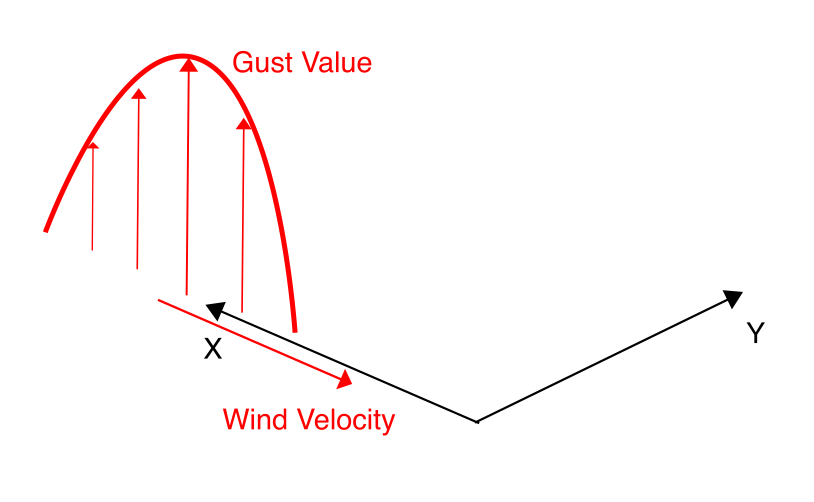
\includegraphics[width=0.85\linewidth]{Images/Gust.png}
    \caption{Gust Movement}
    \label{fig:Gust}
\end{figure}

\begin{itemize}
    \item Case 1: -10 m/s Gust in X-axis: Gust wind moves backward along the X-axis with 1 m/s.
    \item Case 2: 10 m/s Gust in X-axis: Gust wind moves forward along the X-axis with 1 m/s.
    \item Case 3: 10 m/s Gust in Y-axis: Gust wind moves forward along the Y-axis with 1 m/s.
    \item Case 4: 10 m/s Gust in Z-axis: Gust wind moves backward along the X-axis with 1 m/s.
\end{itemize}

Figures \ref{fig:fixed -x}, \ref{fig:fixed x}, \ref{fig:fixed y}, and \ref{fig:fixed z} depict the change of reaction force and moment of the joint at the mass center.

In Chapter \ref{ch:chapter1}, Section \ref{section:Aerodynamic elements}, aerodynamic force and moment generated by the wing are introduced, and in Section \ref{section:force elements}, the thrust force generated by the propeller is introduced by Equation \ref{eq:thrust}. Based on these equations, reaction force and moment acting on the clamp joint can be analyzed.

\begin{figure}[htbp]
    \centering
    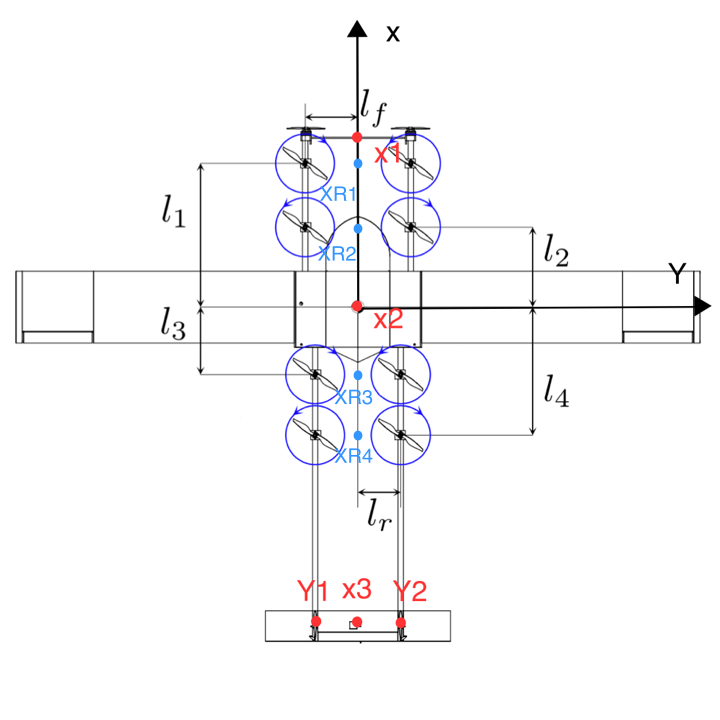
\includegraphics[width=0.75\linewidth]{Images/Gust_Position.png}
    \caption{Gust Position}
    \label{fig:Gust position}
\end{figure}

\textbf{Case 1:} In Figure \ref{fig:fixed -x}, as depicted in Figure \ref{fig:Gust position}, the gust moves backward along the X-axis. When the gust arrives at different positions, the force and moment change. When the gust passes through position \textit{X1}, the thrust force generated by the propeller decreases due to gust airflow. Then, when the gust arrives at position \textit{X2}, the main wing generates a large lift and drag due to the gust. Finally, when the gust arrives at position \textit{X3}, the tail wing generates lift and drag. Due to the smaller pitch angle and wing surface compared to the main wing, the effect on the reaction force and moment changes less. The values are summarized in Table \ref{tab:verify -x}.

\textbf{Case 2:} Similarly, in Figure \ref{fig:fixed x}, the gust moves forward along the X-axis. The gust would arrive at position \textit{X3} first, then arrive at position \textit{X2}. The computed values are summarized in Table \ref{tab:verify x}.

\textbf{Case 3:} In Figure \ref{fig:fixed y}, the reaction force and moment are generated due to the vertical tail wing. The gust moves forward along the Y-axis, arriving at position \textit{Y1} first, then position \textit{Y2}. The computed values are summarized in Table \ref{tab:verify y}.

\textbf{Case 4:} In Figure \ref{fig:fixed z}, the gust moves backward along the X-axis, which is Similar with case 1, when the gust arrives at position \textit{X2}, the main wing generates a large lift and drag due to the gust, and when the gust arrives at position \textit{X3}. When the gust passes through position of each vertical propeller, the thrust force generated by the propeller increase in turn due to gust airflow. The computed values are summarized in Table \ref{tab:verify z}.

Comparing the computed values and measured values in simulation, due to an error between hand-computed and simulation values below $1 \times 10^{-6}$, they can be considered equivalent.

\begin{table}
    \centering
    \begin{tabular}{ccccc}
    \hline
        Position & Time Delay (s) & $F_{X}$ (N) & $F_{Z}$ (N) & $M_{Y}$ (N*m) \\
    \hline
        before X1   &       & 5.1002 & 0        & 0 \\
        X1          &       & 2.0135 & 0        & 0 \\
        X2          & 0.4960 & 1.0533 & -24.8717 & 0.899845 \\
        X3          & 1.08  & 0.9507 & -25.6849  & 0.0801132\\
    \hline
    \end{tabular}
    \caption{Joint reaction force, moment change and time delay when gust move backward along X-axis}
    \label{tab:verify -x}
\end{table}

\begin{table}
    \centering
    \begin{tabular}{ccccc}
    \hline
        Position & Time Delay (s) & $F_{X}$ (N) & $F_{Z}$ (N) & $M_{Y}$ (N*m) \\
    \hline
        before X3   &       & 5.1004 & 0        & 0 \\
        X3          &       & 5.31  & 1.09691 & 1.15002 \\
        X2          & 1.08  & 7.17  & 15.4294 & 1.5691 \\
        X1          & 0.4960 & 9.16 & 15.4294 & 1.5691 \\
    \hline
    \end{tabular}
    \caption{Joint reaction force, moment change and time delay change when gust move forward along X-axis}
    \label{tab:verify x}
\end{table}

\begin{table}
    \centering
    \begin{tabular}{cccccc}
    \hline
        Position & Time Delay (s) & $F_{X}$ (N) & $F_{Y}$ (N)& $M_{X}$ (N*m) & $M_{Z}$ (N*m) \\
    \hline
        before Y1   &           & 5.1004 & 0        & 0         & 0 \\
        Y1          &           & 5.1689 & -2.20449 & -0.1962   & 2.28083 \\
        Y2          & 0.2630    & 5.2368 & -4.40897 & -0.392398 & 4.57972 \\
    \hline
    \end{tabular}
    \caption{Joint reaction force, moment change and time delay when gust move forward along Y-axis}
    \label{tab:verify y}
\end{table}
% REDONE
\begin{table}
    \centering
    \begin{tabular}{ccccc}
    \hline
        Position & Time Delay (s) & $F_{X}$ (N) & $F_{Z}$ (N) & $M_{Y}$ (N*m)\\
    \hline
        before XR1  &       &  0        & -65.68    & 2.34        \\       
        XR1         &       &  0        & -69.45    & 3.91         \\   
        XR2         & 0.146 &  0        & -73.22   & 4.92        \\       
        X2          & 0.267 &  -1.593   & -142.889  & 5.2433     \\       
        XR3         & 0.191 &  -1.593   & -146.664   & 4.4889      \\       
        XR4         & 0.146 &  -1.593   & -150.439  &  3.195    \\           
        X3          & 0.67  &  -1.66    & -157.54   &  -4.185    \\           
    \hline
    \end{tabular}
    \caption{Joint reaction force, moment change and time delay when gust move forward along Z-axis}
    \label{tab:verify z}
\end{table}

\begin{figure}[htbp]
  \centering
  \begin{minipage}[b]{0.3\textwidth}
    \centering
    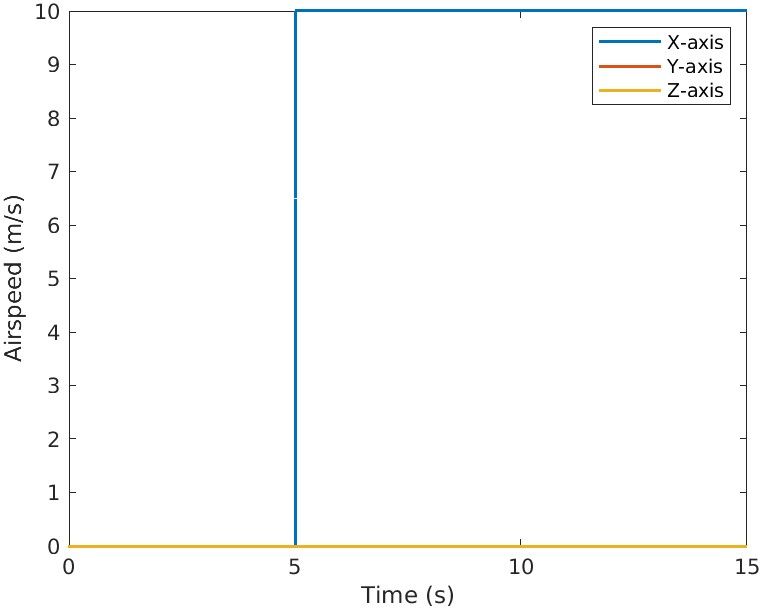
\includegraphics[width=\textwidth]{Images/Gust/FIXED/1 airspeed_1.jpg}
    \caption*{\textit{True Airspeed}}
  \end{minipage}
  \hfil
  \begin{minipage}[b]{0.3\textwidth}
    \centering
    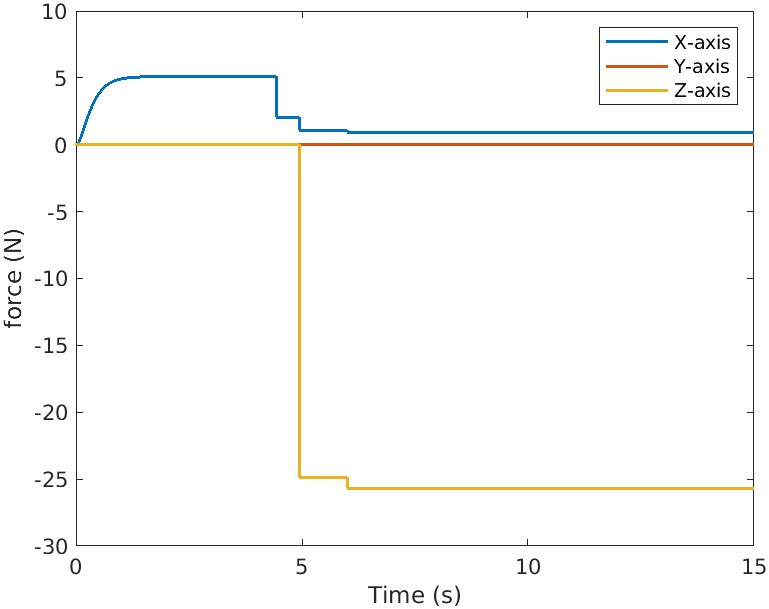
\includegraphics[width=\textwidth]{Images/Gust/FIXED/2 force_1.jpg}
    \caption*{\textit{Reaction Force}}
  \end{minipage}
  \hfil
  \begin{minipage}[b]{0.3\textwidth}
    \centering
    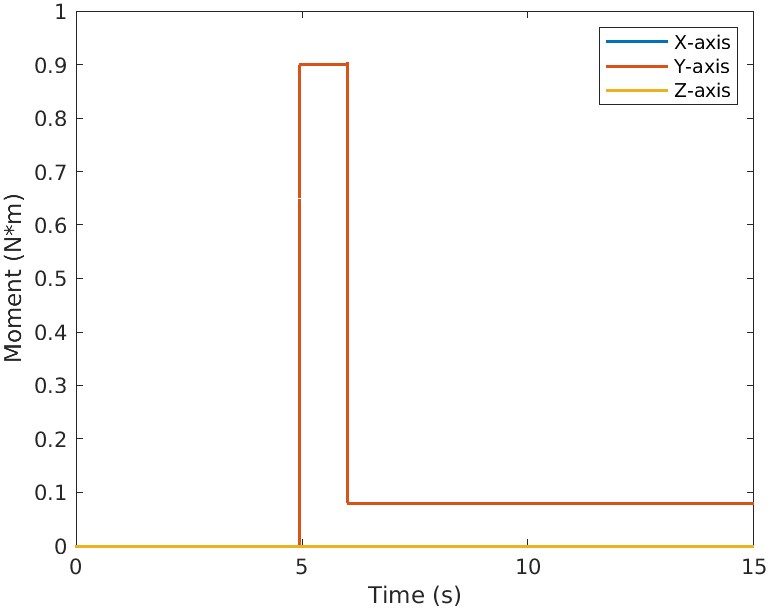
\includegraphics[width=\textwidth]{Images/Gust/FIXED/3 moment_1.jpg}
    \caption*{\textit{Reaction Moment}}
  \end{minipage}
  \caption{Status in mass center of airframe when step gust move backward along X-axis}
  \label{fig:fixed -x}
\end{figure}

\begin{figure}[htbp]
  \centering
  \begin{minipage}[b]{0.3\textwidth}
    \centering
    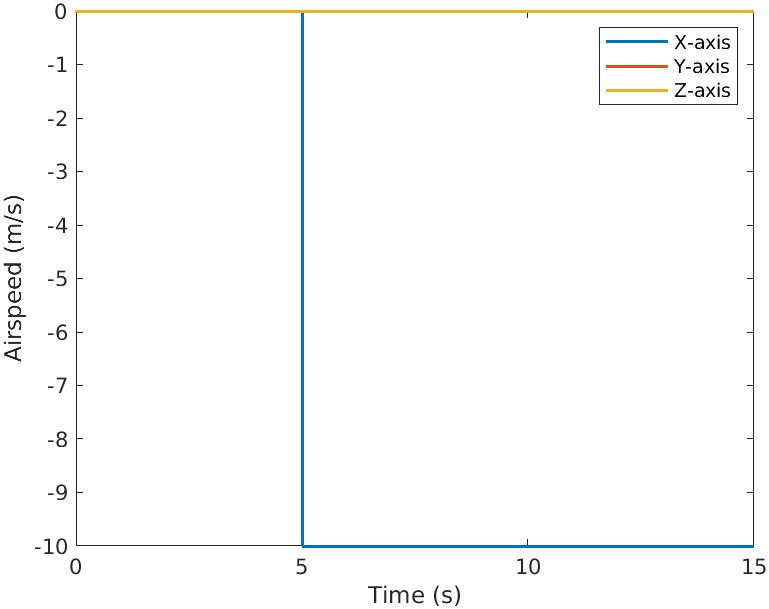
\includegraphics[width=\textwidth]{Images/Gust/FIXED/1 airspeed_2.jpg}
    \caption*{\textit{True Airspeed}}
  \end{minipage}
  \hfil
  \begin{minipage}[b]{0.3\textwidth}
    \centering
    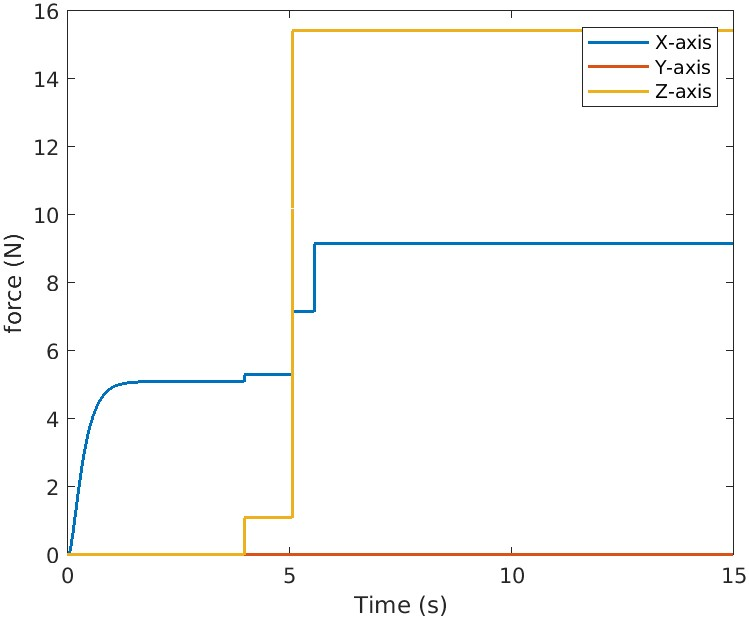
\includegraphics[width=\textwidth]{Images/Gust/FIXED/2 force_2.jpg}
    \caption*{\textit{Reaction Force}}
  \end{minipage}
  \hfil
  \begin{minipage}[b]{0.3\textwidth}
    \centering
    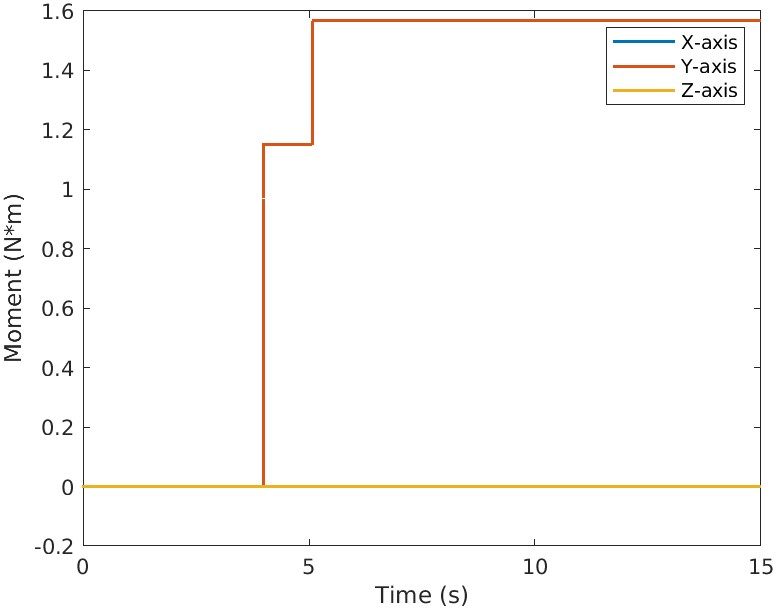
\includegraphics[width=\textwidth]{Images/Gust/FIXED/3 moment_2.jpg}
    \caption*{\textit{Reaction Moment}}
  \end{minipage}
  \caption{Status in mass center of airframe when step gust move forward along X-axis}
  \label{fig:fixed x}
\end{figure}

\begin{figure}[htbp]
  \centering
  \begin{minipage}[b]{0.3\textwidth}
    \centering
    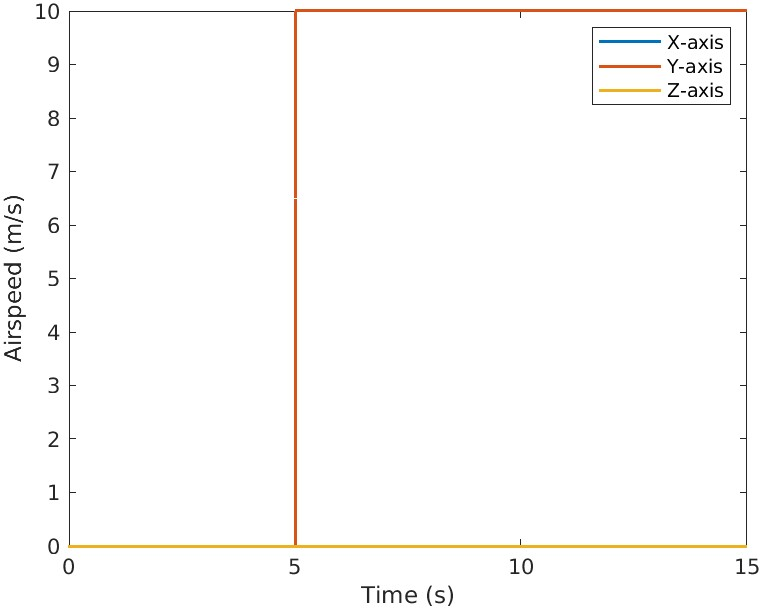
\includegraphics[width=\textwidth]{Images/Gust/FIXED/1 airspeed_3.jpg}
    \caption*{\textit{True Airspeed}}
  \end{minipage}
  \hfil
  \begin{minipage}[b]{0.3\textwidth}
    \centering
    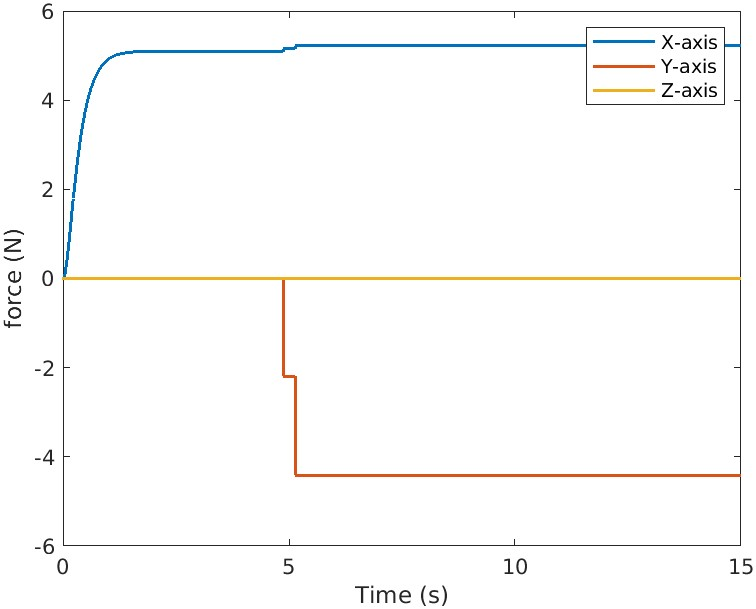
\includegraphics[width=\textwidth]{Images/Gust/FIXED/2 force_3.jpg}
    \caption*{\textit{Reaction Force}}
  \end{minipage}
  \hfil
  \begin{minipage}[b]{0.3\textwidth}
    \centering
    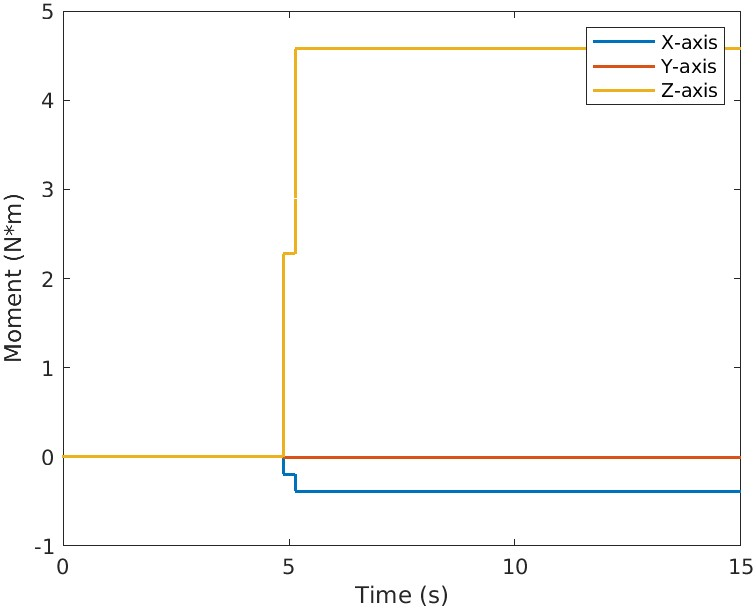
\includegraphics[width=\textwidth]{Images/Gust/FIXED/3 moment_3.jpg}
    \caption*{\textit{Reaction Moment}}
  \end{minipage}
  \caption{Status in mass center of airframe when step gust move forward along Y-axis}
  \label{fig:fixed y}
\end{figure}
% REDONE
\begin{figure}[htbp]
  \centering
  \begin{minipage}[b]{0.3\textwidth}
    \centering
    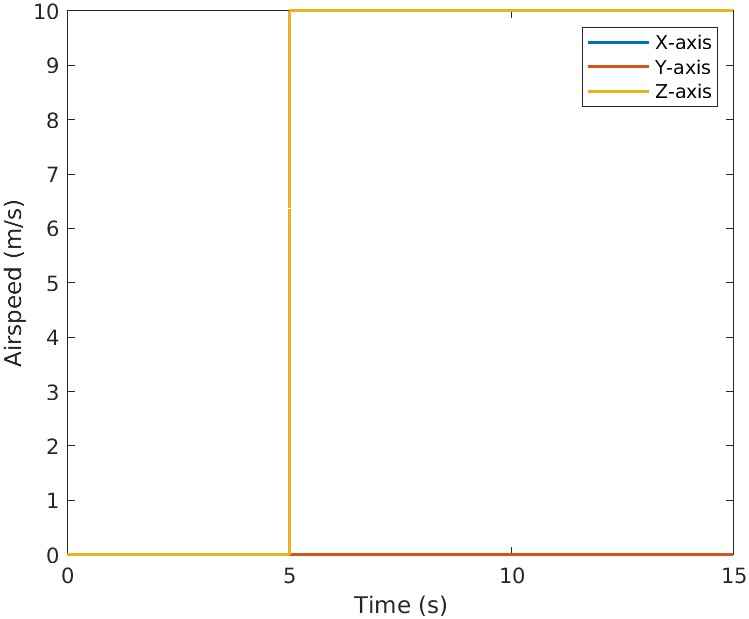
\includegraphics[width=\textwidth]{Images/Gust/FIXED/1 airspeed_4.jpg}
    \caption*{\textit{True Airspeed}}
  \end{minipage}
  \hfil
  \begin{minipage}[b]{0.3\textwidth}
    \centering
    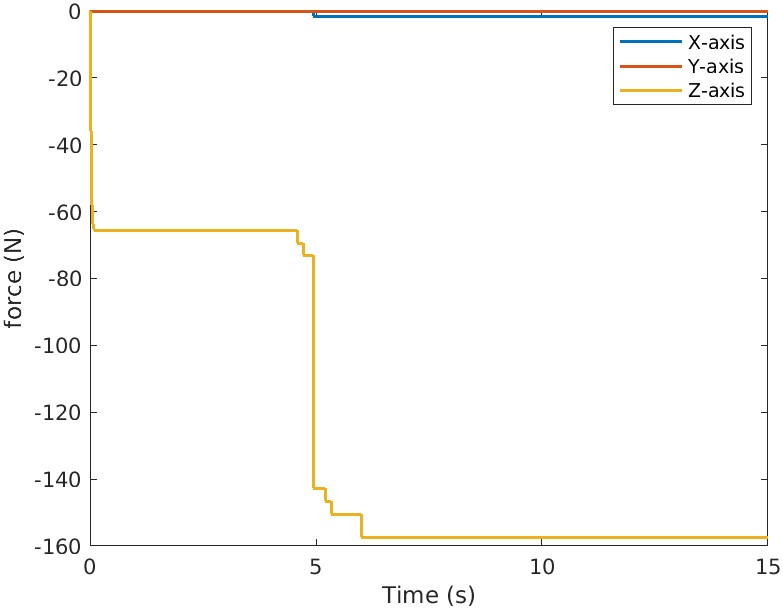
\includegraphics[width=\textwidth]{Images/Gust/FIXED/2 force_4.jpg}
    \caption*{\textit{Reaction Force}}
  \end{minipage}
  \hfil
  \begin{minipage}[b]{0.3\textwidth}
    \centering
    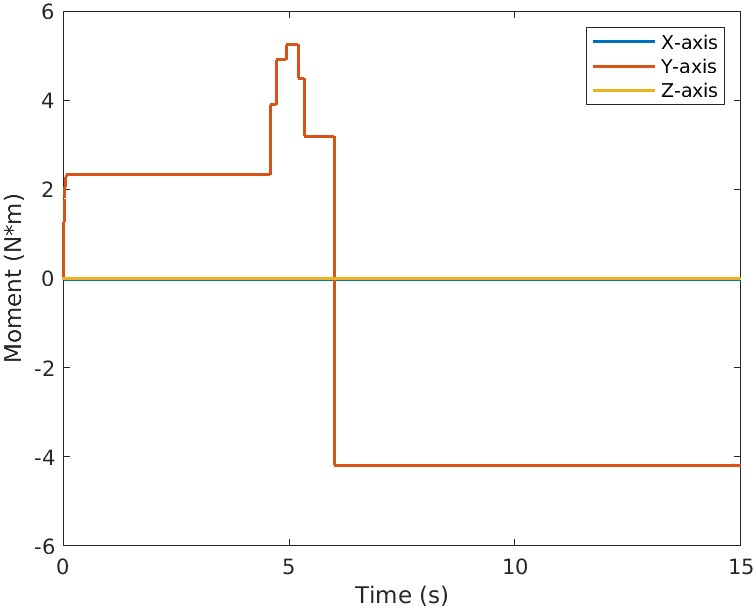
\includegraphics[width=\textwidth]{Images/Gust/FIXED/3 moment_4.jpg}
    \caption*{\textit{Reaction Moment}}
  \end{minipage}
  \caption{Status in mass center of airframe when step gust move forward along Z-axis}
  \label{fig:fixed z}
\end{figure}

\subsection{Gust Experimental Test Procedure and Setup}

When comparing this specific UAV to traditional helicopters and multi-copter UAVs, it is essential to consider its additional wing structure, which can significantly influence its performance in gusty winds. According to ADS-33 regulations, the drone undergoes gust testing under various wind conditions, ranging from calm (0-5 knots, 0-2.57 m/s), light (10-15 knot, 5.14-7.72 m/s)  moderate (25-35 knots, 12.86-18.01 m/s). While most missions can be accomplished in calm or light winds, the drone is specifically scrutinized for its performance in gusts across all three axes, Since the unit of wind speed in ADS-33E is knots, the unit of wind speed in this section is still knots.

In the \textit{Air properties} element of MBDyn, various gust wind models are available for selection. The Front 1D type stands out as the most suitable model for simulating gusts in a realistic environment. To accurately replicate real-world conditions during drone flights, the cosine function is employed to depict the behavior of gusts. Gusty winds for drones predominantly manifest in two forms: pulse gusty winds and constant gusty winds. For pulse gusts, a single cycle lasting 5 seconds is utilized, while a half cycle is employed for step gusts to transition the gust value from 0 knots to the desired gust value. This meticulous approach ensures the precision and reliability of our simulations. Gust wind is programmed to reach the original center of the global frame precisely 5 seconds into the simulation when the drone operates in multi-copter mode and remains in hover status.

During multi-copter mode operations, the control system is configured to focus solely on gust resistance testing, as this particular test case primarily evaluates the aircraft's ability to withstand gusts. Therefore, position hold control can be disregarded. In gust testing, multi-copter mode exclusively employs velocity control after climbing to required altitude, with all velocity setpoints set to null. Additionally, yaw angle control is set to null to maintain the aircraft's heading direction. The total experimental test cases for gust resistance are summarized in Table \ref{tab:gust VTOL}.

\begin{sidewaystable}[htbp]
    \centering
    \begin{tabular}{ccccc}
    \hline
        Control Mode & Gust Type & Gust Direction & Gust Value (knots) & Move Direction \\
        \hline
        multicopter Mode & Step & X-axis & -35 & Backward along X-axis \\
        multicopter Mode & Step & X-axis & 10 & Forward along X-axis \\
        multicopter Mode & Step & Y-axis & 5 & Forward along Y-axis \\
        multicopter Mode & Step & Y-axis & 5 & Backward along X-axis \\
        multicopter Mode & Step & Z-axis & 15 & Backward along X-axis \\
        \hline
        multicopter Mode & Pulse & X-axis & -35 & Forward along X-axis \\
        multicopter Mode & Pulse & X-axis & 20 & Backward along X-axis \\
        multicopter Mode & Pulse & Y-axis & 5 & Forward along Y-axis \\
        multicopter Mode & Pulse & Y-axis & 5 & Backward along X-axis \\
        multicopter Mode & Pulse & Z-axis & 15 & Backward along X-axis \\
        \hline
        Fixed-wing Mode & Pulse & X-axis & -15 & Backward along X-axis \\
        Fixed-wing Mode & Pulse & X-axis & -5 & forward along X-axis \\
        Fixed-wing Mode & Pulse & Y-axis & 15 & Backward along X-axis \\
        Fixed-wing Mode & Pulse & Z-axis & 15 & Backward along X-axis \\
    \hline
    \end{tabular}
    \caption{Gust Test of Aircraft in Multicopter Mode}
    \label{tab:gust VTOL}
\end{sidewaystable}

\subsubsection{Step Gust Test for Aircraft in Multi-Copter Mode}

The drone's response to a gust of wind moving along the X-axis from positive to negative directions illustrates in Figure \ref{fig:VTOL step -x} . This gust induces additional drag and lift on the drone's wing, resulting in a slight increase in altitude and backward movement. The drone exhibits resilience against moderate wind gusts under these conditions.

Conversely, in Figure \ref{fig:VTOL step x}, when a gust of wind moves forward along the X-axis, instability in the yaw angle, coupled with the effects of rolling and pitch angles, may cause the drone to lose control. The maximum tolerable gust under this circumstance is 10 knots.

Gusts along the Y-axis, depicted in Figures \ref{fig:VTOL step yy} and \ref{fig:VTOL step xy}, exert significant torque on the vertical tail wing, resulting in substantial yaw angle changes. However, the torque generated by the vertical propeller is limited, rendering the drone unable to withstand high gusts exceeding 5 knots.

Figure \ref{fig:VTOL step z} portrays the impact of gusts along the Z-axis. The main wing and horizontal tail experience elevated drag and lift, necessitating significant pitch angle adjustments to maintain force and moment distribution. Excessive gusts can induce large pitch angle changes, potentially resulting in loss of control. The maximum tolerable gust along the Z-axis is 15 knots.

In conclusion, while the aircraft demonstrates good resistance performance against gusts in the X-axis and Z-axis, its resistance capability is comparatively lower when gusts occur along the Y-axis, primarily due to the structural characteristics of the vertical tail wing.

\begin{figure}[htbp]
  \centering
  \begin{minipage}[b]{0.45\textwidth}
    \centering
    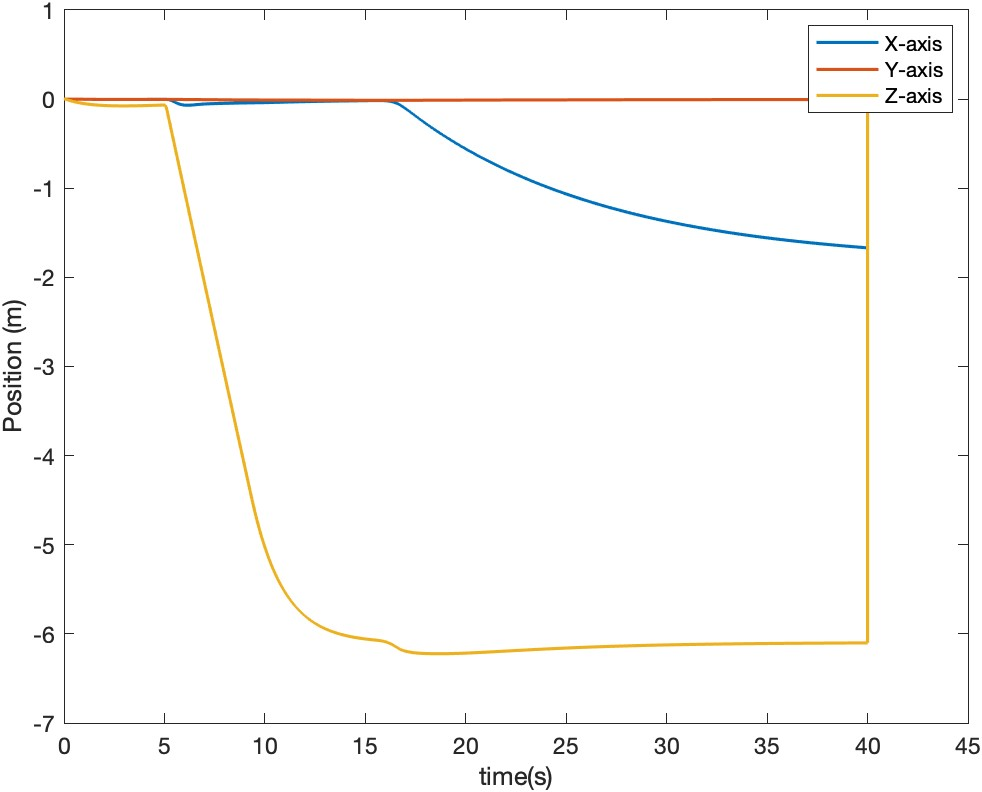
\includegraphics[width=\textwidth]{Images/Gust/VTOL step/1 position_1.jpg}
    \caption*{\textit{Position}}
  \end{minipage}
  \hfil
  \begin{minipage}[b]{0.45\textwidth}
    \centering
    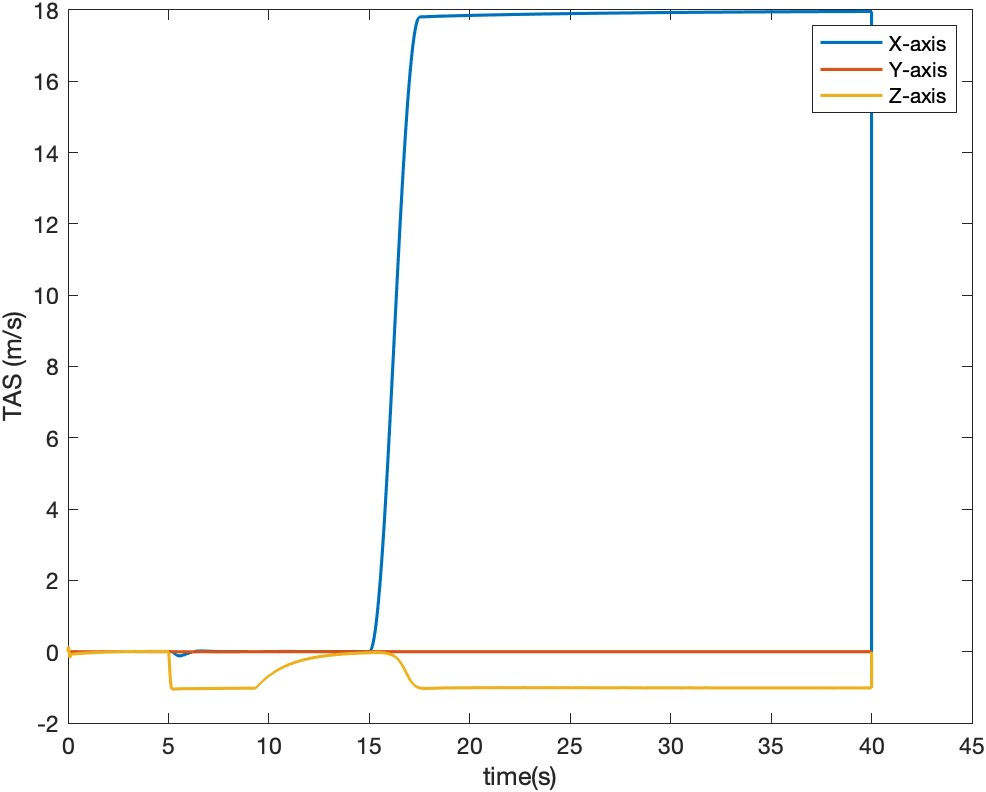
\includegraphics[width=\textwidth]{Images/Gust/VTOL step/2 airspeed_1.jpg}
    \caption*{\textit{True Airspeed}}
  \end{minipage}
  \begin{minipage}[b]{0.45\textwidth}
    \centering
    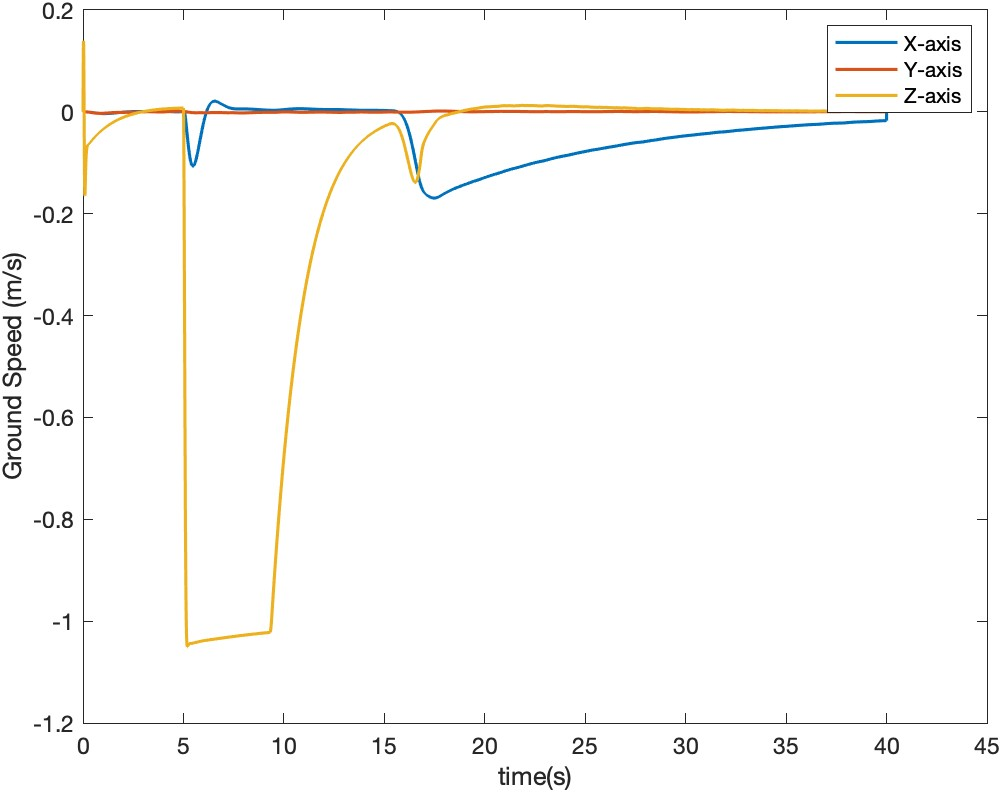
\includegraphics[width=\textwidth]{Images/Gust/VTOL step/3 groundspeed_1.jpg}
    \caption*{\textit{Ground Speed}}
  \end{minipage}
  \hfil
  \begin{minipage}[b]{0.45\textwidth}
    \centering
    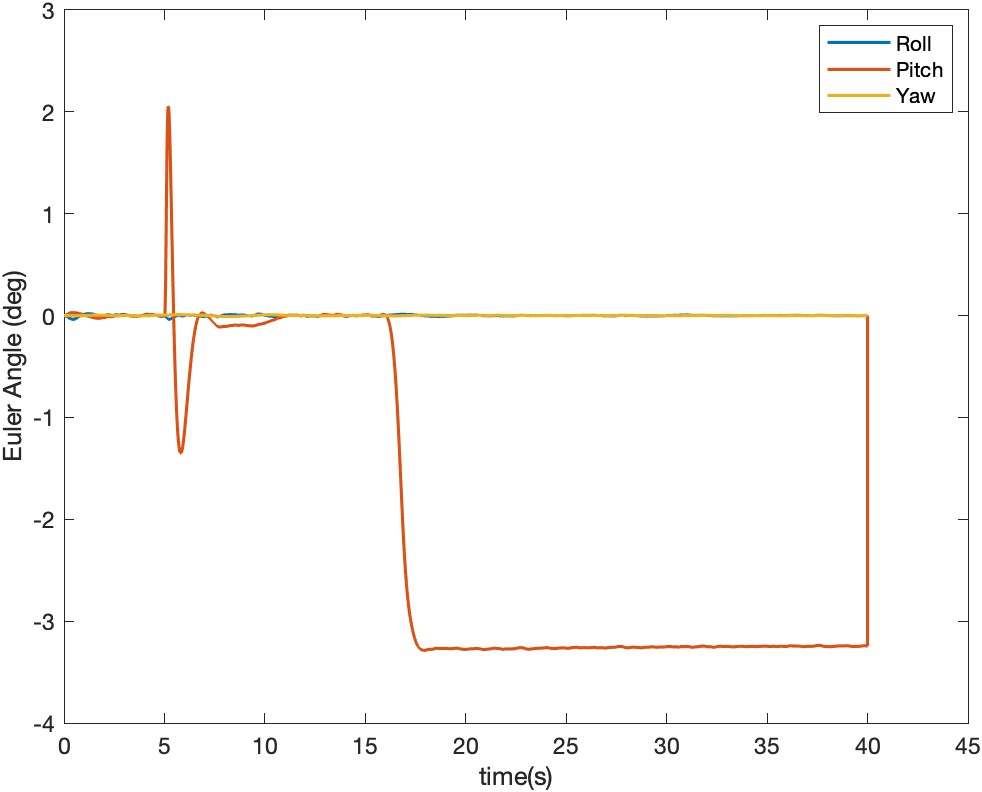
\includegraphics[width=\textwidth]{Images/Gust/VTOL step/4 EulerAngle_1.jpg}
    \caption*{\textit{Euler Angle}}
  \end{minipage}
  \caption{Status of aircraft in multicopter mode when step gust in negative X-axis move backward along X-axis}
  \label{fig:VTOL step -x}
\end{figure}

\begin{figure}[htbp]
  \centering
  \begin{minipage}[b]{0.45\textwidth}
    \centering
    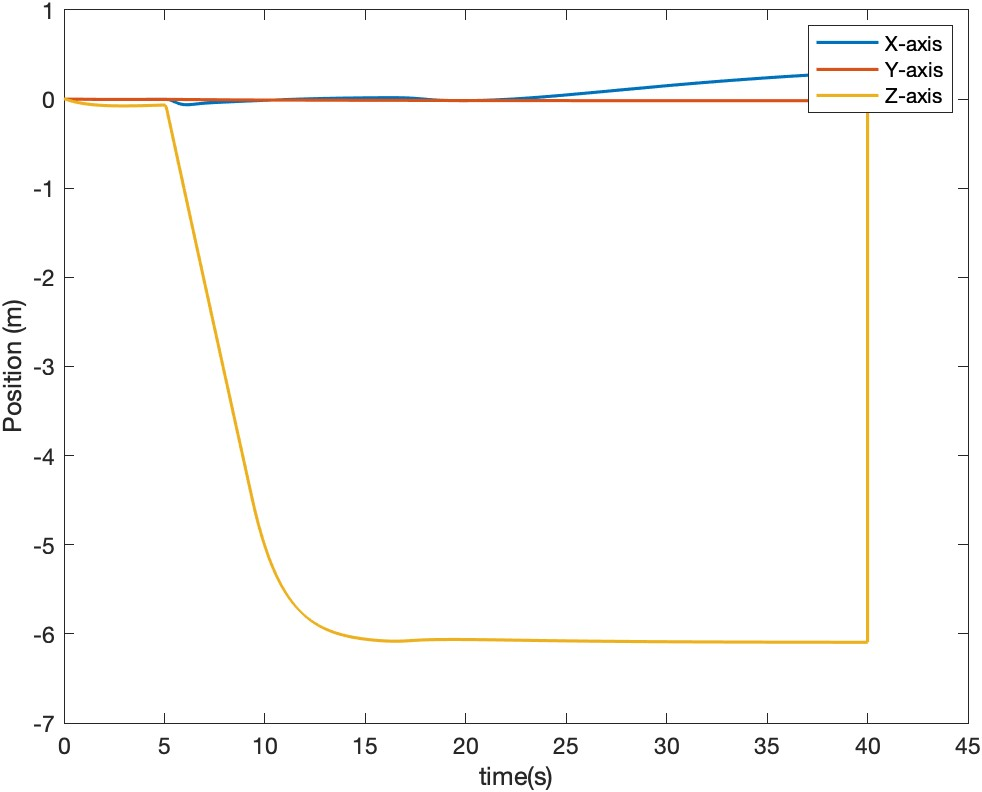
\includegraphics[width=\textwidth]{Images/Gust/VTOL step/1 position_2.jpg}
    \caption*{\textit{Position}}
  \end{minipage}
  \hfil
  \begin{minipage}[b]{0.45\textwidth}
    \centering
    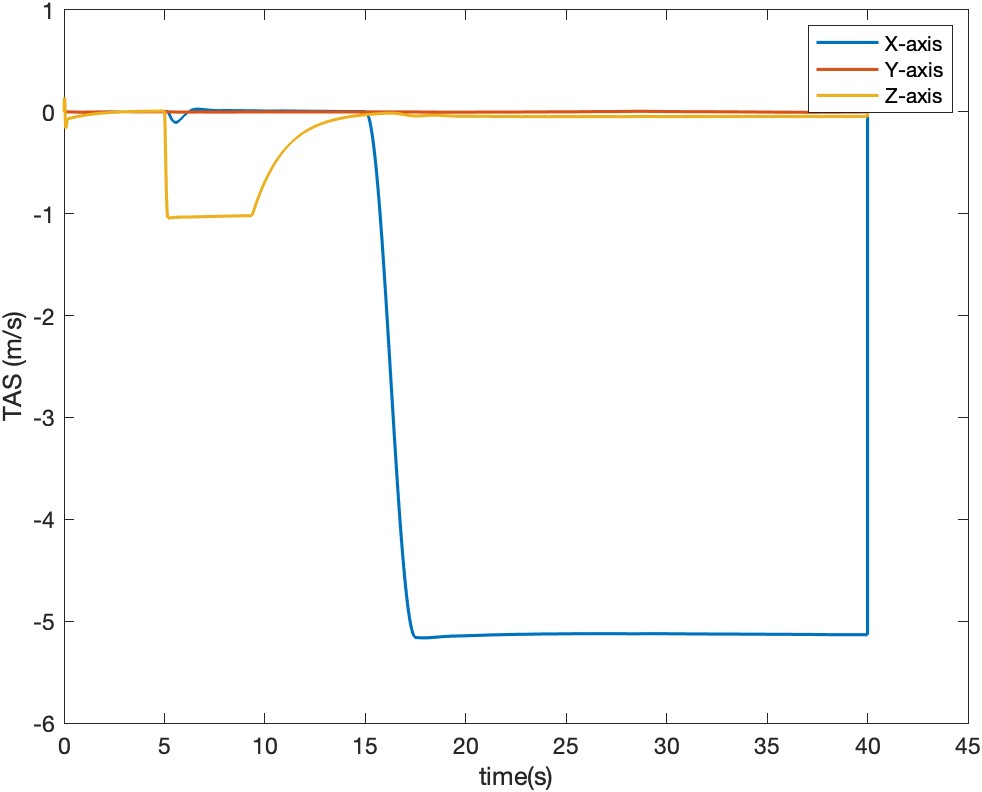
\includegraphics[width=\textwidth]{Images/Gust/VTOL step/2 airspeed_2.jpg}
    \caption*{\textit{True Airspeed}}
  \end{minipage}
  \begin{minipage}[b]{0.45\textwidth}
    \centering
    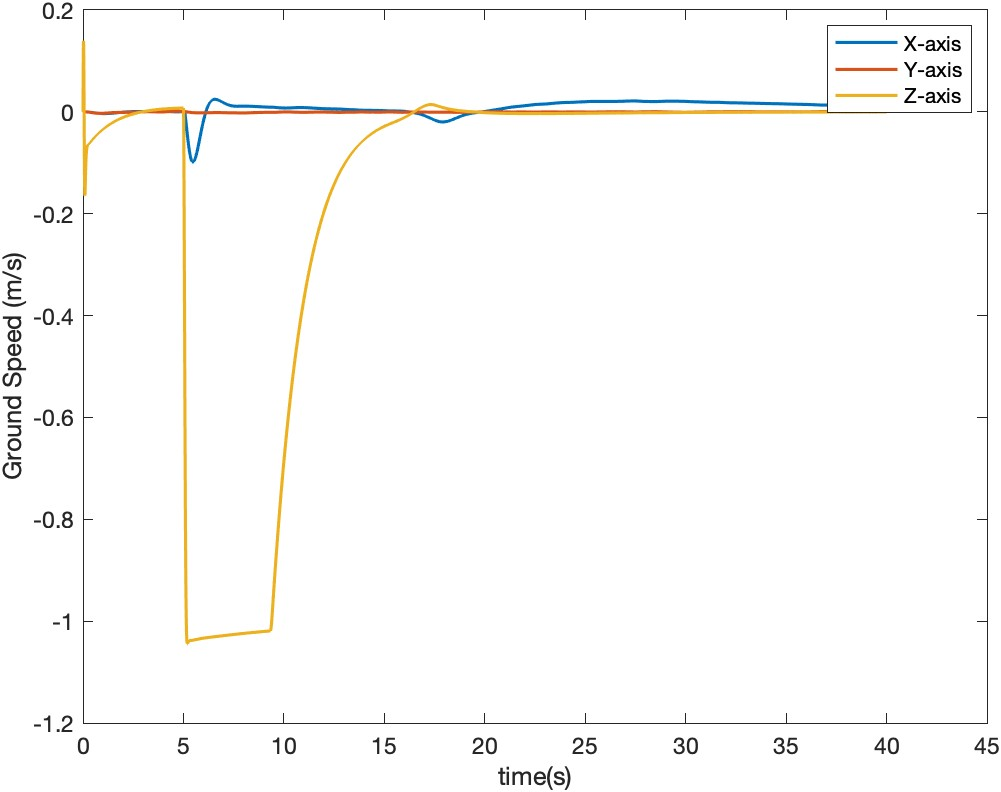
\includegraphics[width=\textwidth]{Images/Gust/VTOL step/3 groundspeed_2.jpg}
    \caption*{\textit{Ground Speed}}
  \end{minipage}
  \hfil
  \begin{minipage}[b]{0.45\textwidth}
    \centering
    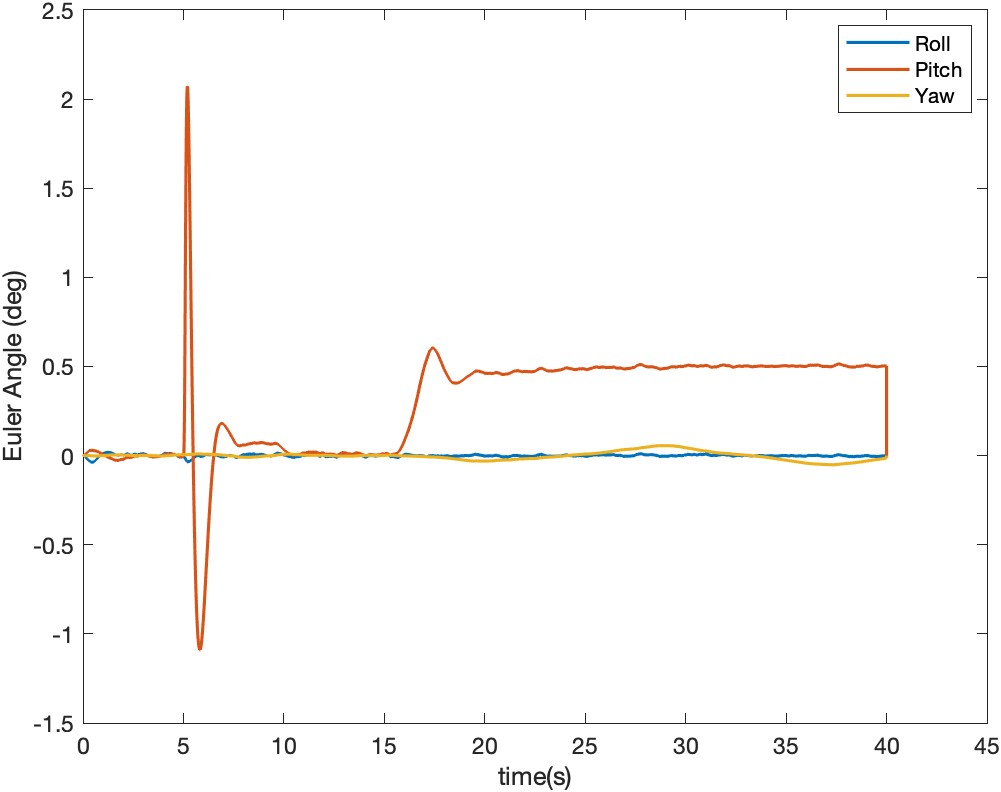
\includegraphics[width=\textwidth]{Images/Gust/VTOL step/4 EulerAngle_2.jpg}
    \caption*{\textit{Euler Angle}}
  \end{minipage}
  \caption{Status of aircraft in multicopter mode when step gust in positive X-axis move forward along X-axis}
  \label{fig:VTOL step x}
\end{figure}

\begin{figure}[htbp]
  \centering
  \begin{minipage}[b]{0.45\textwidth}
    \centering
    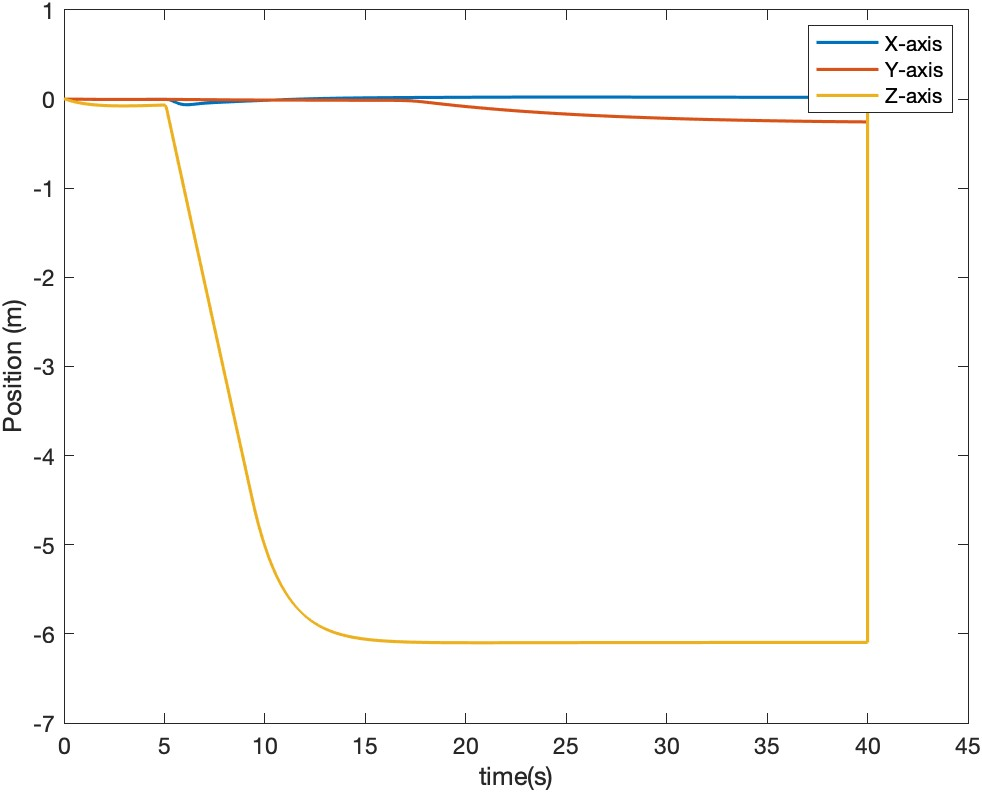
\includegraphics[width=\textwidth]{Images/Gust/VTOL step/1 position_3.jpg}
    \caption*{\textit{Position}}
  \end{minipage}
  \hfil
  \begin{minipage}[b]{0.45\textwidth}
    \centering
    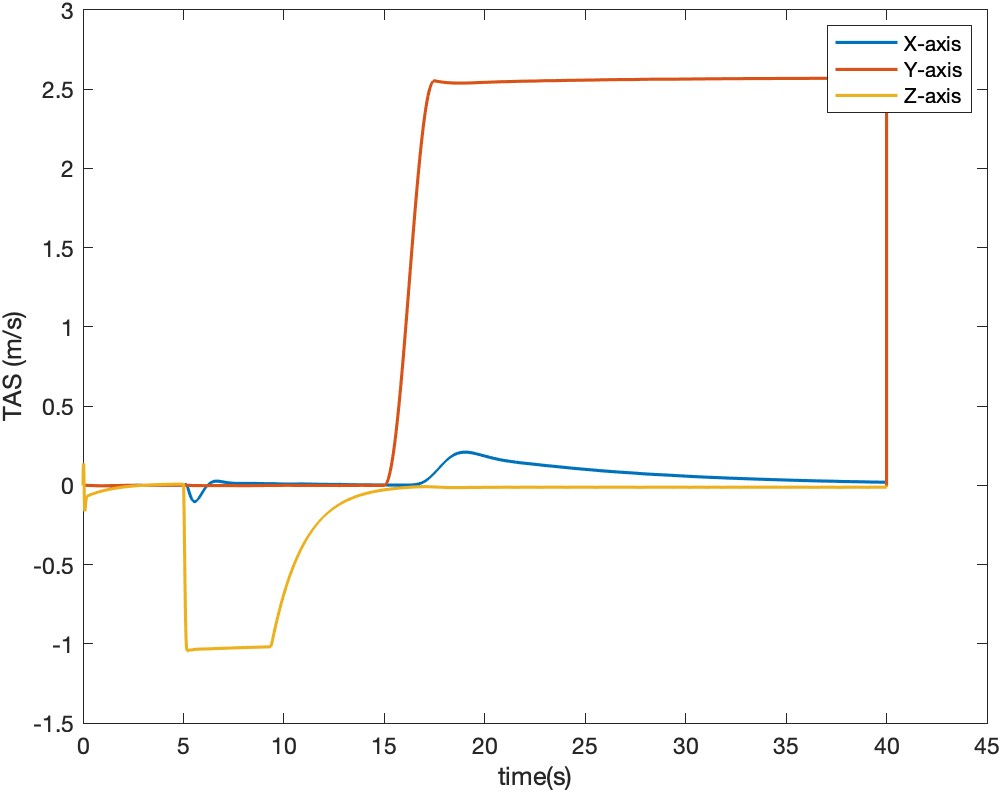
\includegraphics[width=\textwidth]{Images/Gust/VTOL step/2 airspeed_3.jpg}
    \caption*{\textit{True Airspeed}}
  \end{minipage}
  \begin{minipage}[b]{0.45\textwidth}
    \centering
    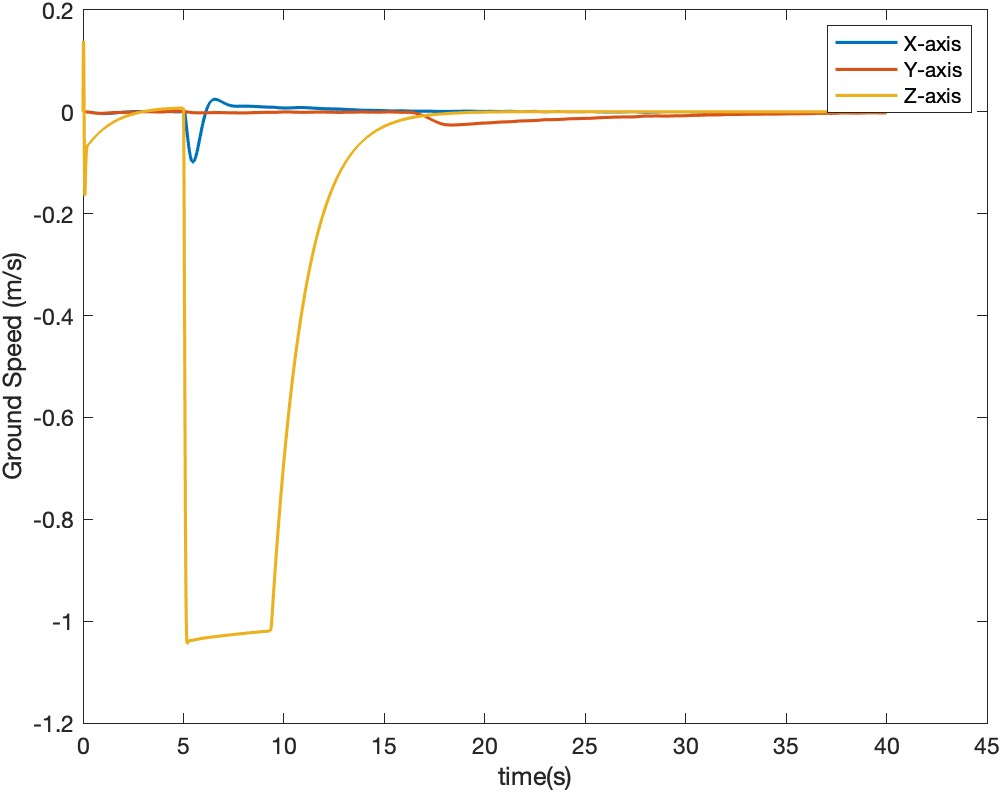
\includegraphics[width=\textwidth]{Images/Gust/VTOL step/3 groundspeed_3.jpg}
    \caption*{\textit{Ground Speed}}
  \end{minipage}
  \hfil
  \begin{minipage}[b]{0.45\textwidth}
    \centering
    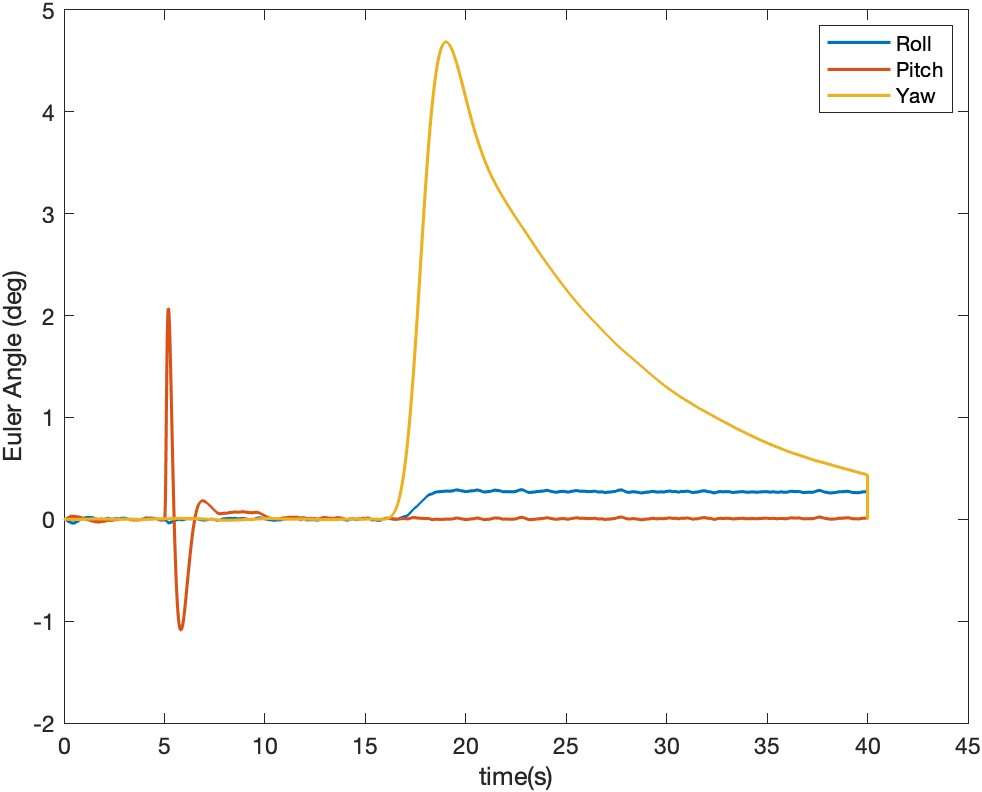
\includegraphics[width=\textwidth]{Images/Gust/VTOL step/4 EulerAngle_3.jpg}
    \caption*{\textit{Euler Angle}}
  \end{minipage}
  \caption{Status of aircraft in multicopter mode when step gust in Y-axis move backward along X-axis}
  \label{fig:VTOL step xy}
\end{figure}

\begin{figure}[htbp]
  \centering
  \begin{minipage}[b]{0.45\textwidth}
    \centering
    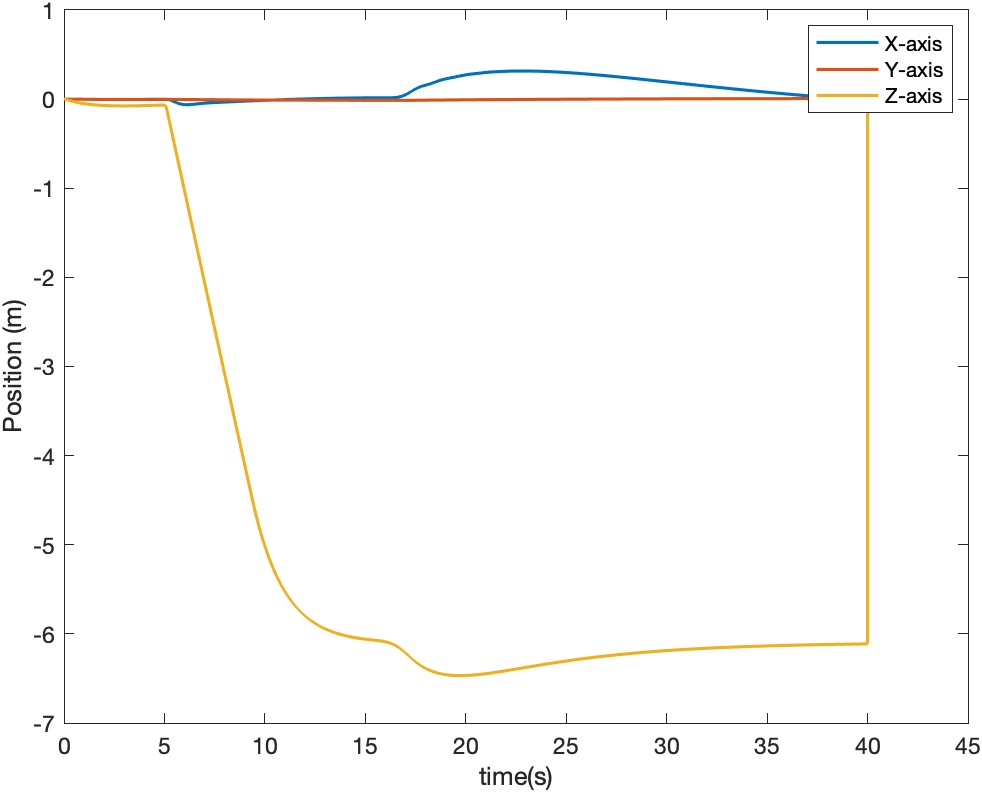
\includegraphics[width=\textwidth]{Images/Gust/VTOL step/1 position_4.jpg}
    \caption*{\textit{Position}}
  \end{minipage}
  \hfil
  \begin{minipage}[b]{0.45\textwidth}
    \centering
    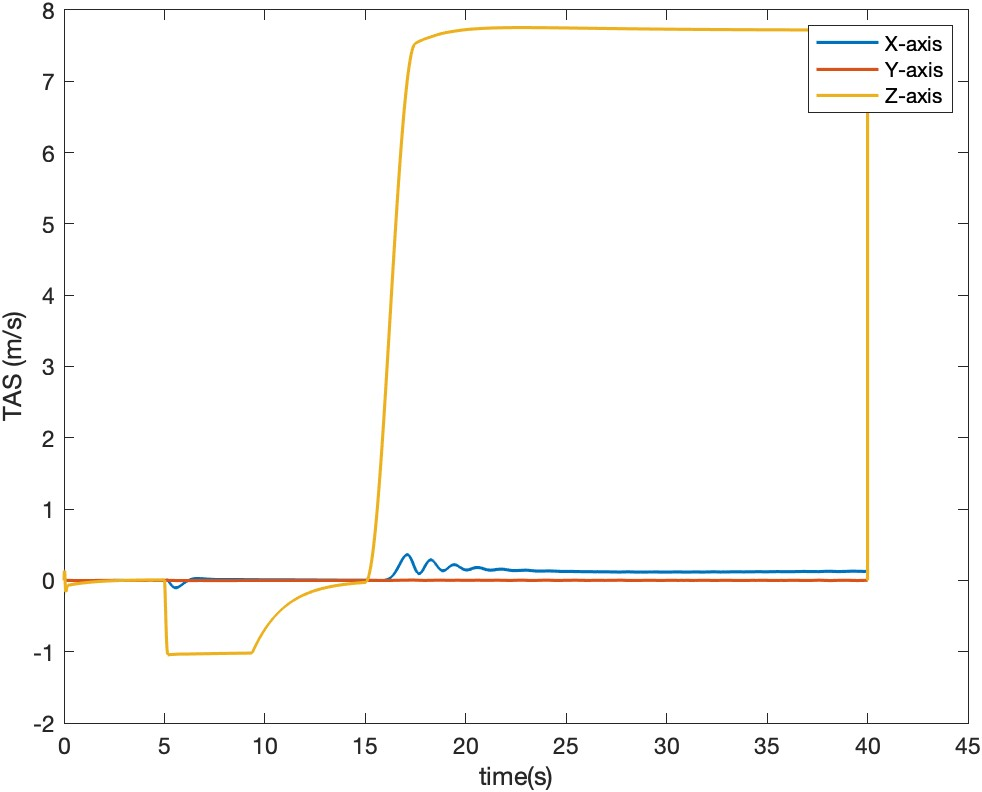
\includegraphics[width=\textwidth]{Images/Gust/VTOL step/2 airspeed_4.jpg}
    \caption*{\textit{True Airspeed}}
  \end{minipage}
  \begin{minipage}[b]{0.45\textwidth}
    \centering
    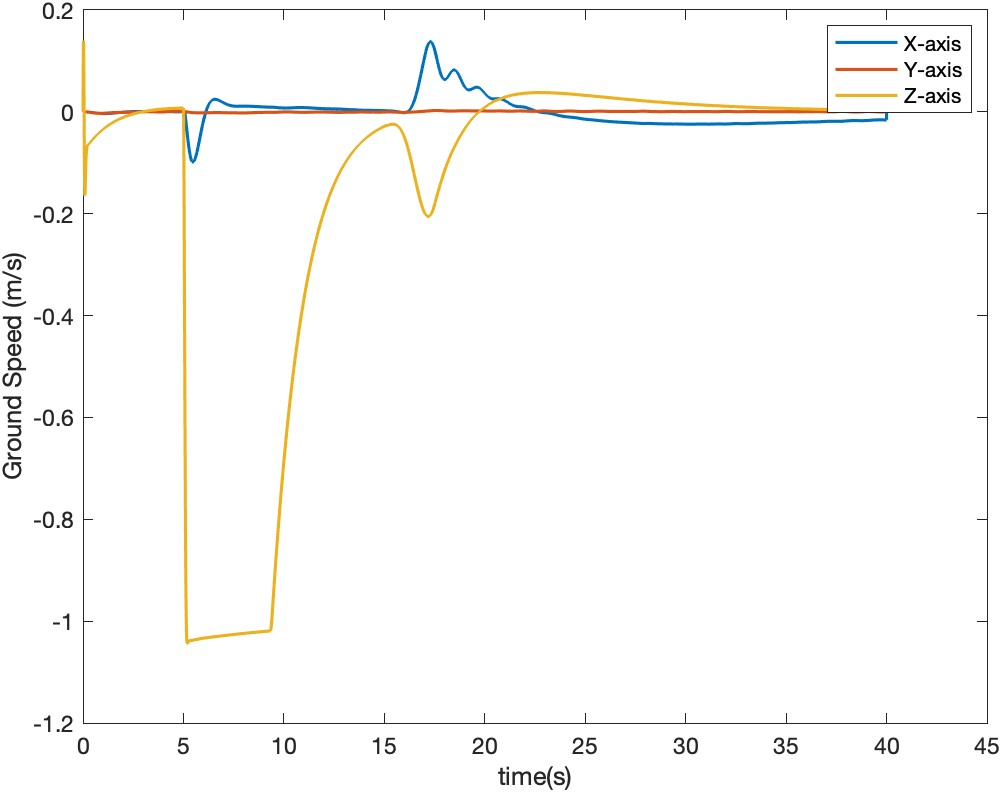
\includegraphics[width=\textwidth]{Images/Gust/VTOL step/3 groundspeed_4.jpg}
    \caption*{\textit{Ground Speed}}
  \end{minipage}
  \hfil
  \begin{minipage}[b]{0.45\textwidth}
    \centering
    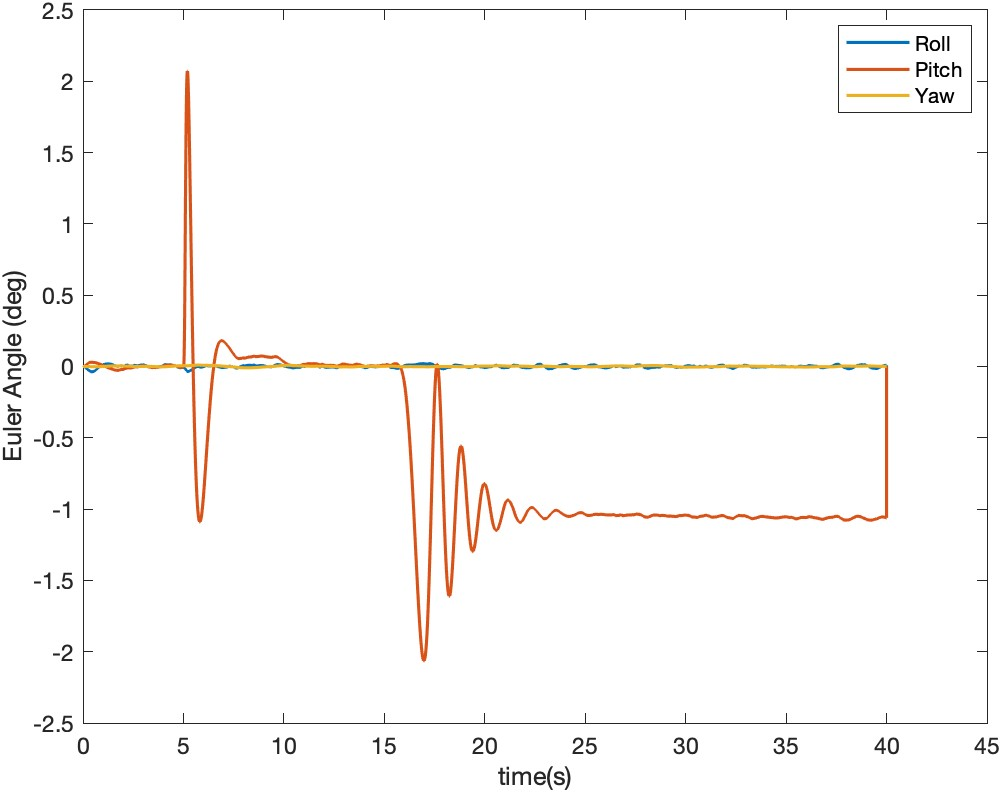
\includegraphics[width=\textwidth]{Images/Gust/VTOL step/4 EulerAngle_4.jpg}
    \caption*{\textit{Euler Angle}}
  \end{minipage}
  \caption{Status of aircraft in multicopter mode when step gust in Z-axis move backward along X-axis}
  \label{fig:VTOL step z}
\end{figure}

\begin{figure}[htbp]
  \centering
  \begin{minipage}[b]{0.45\textwidth}
    \centering
    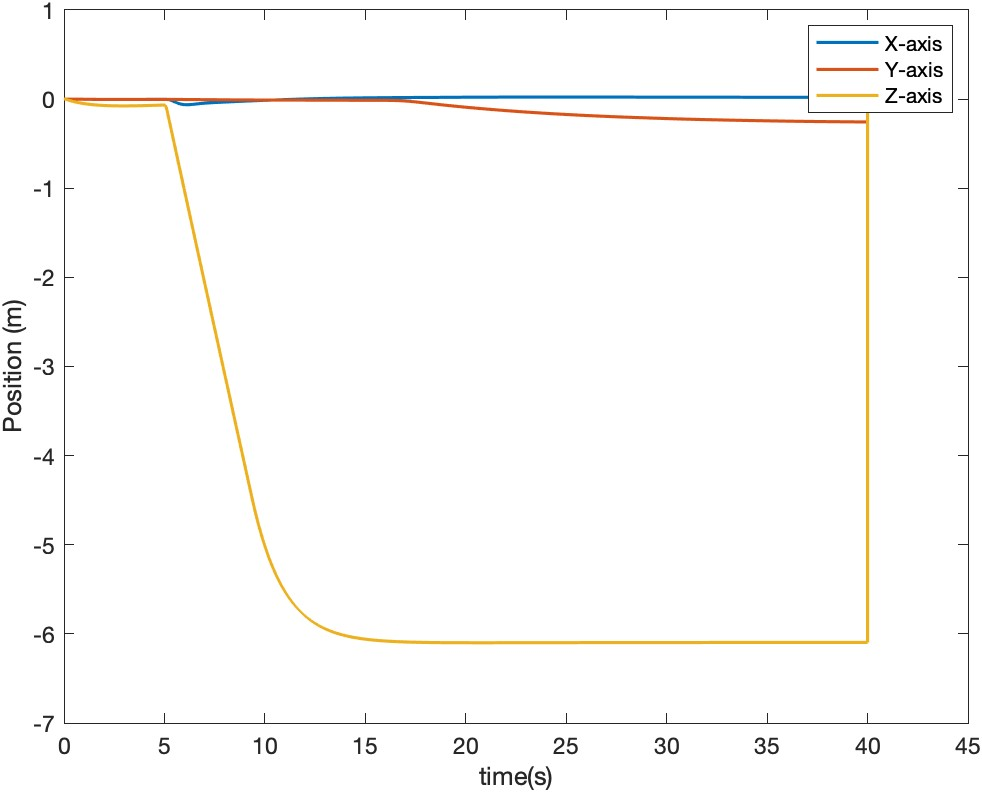
\includegraphics[width=\textwidth]{Images/Gust/VTOL step/1 position_5.jpg}
    \caption*{\textit{Position}}
  \end{minipage}
  \hfil
  \begin{minipage}[b]{0.45\textwidth}
    \centering
    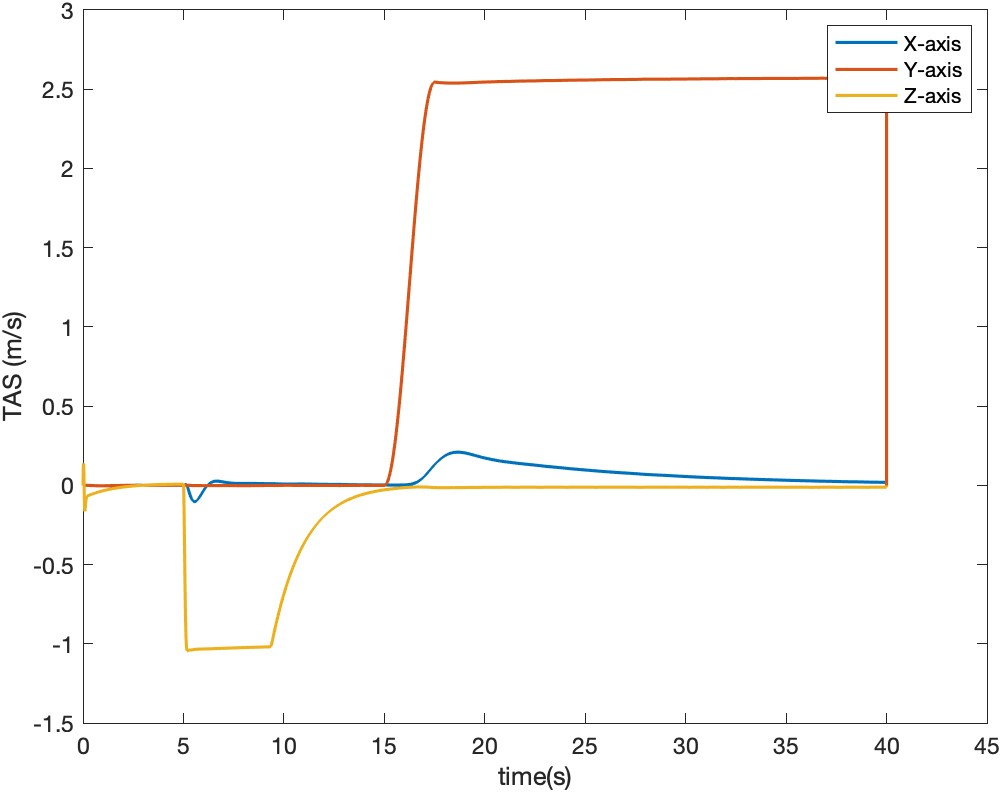
\includegraphics[width=\textwidth]{Images/Gust/VTOL step/2 airspeed_5.jpg}
    \caption*{\textit{True Airspeed}}
  \end{minipage}
  \begin{minipage}[b]{0.45\textwidth}
    \centering
    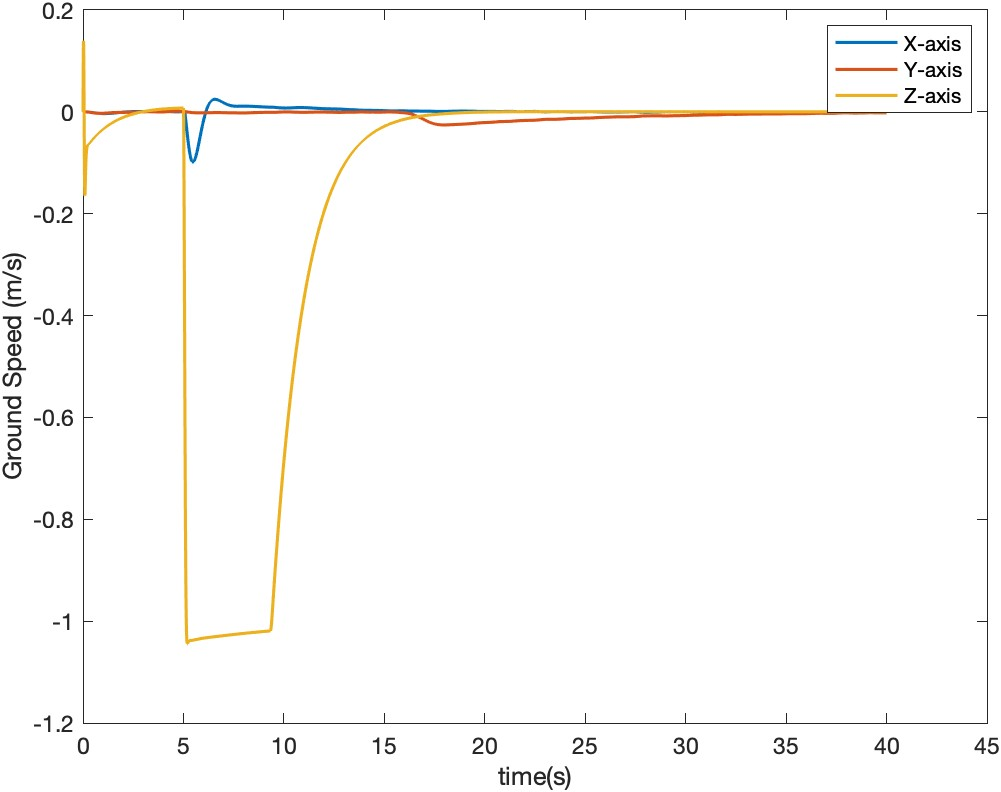
\includegraphics[width=\textwidth]{Images/Gust/VTOL step/3 groundspeed_5.jpg}
    \caption*{\textit{Ground Speed}}
  \end{minipage}
  \hfil
  \begin{minipage}[b]{0.45\textwidth}
    \centering
    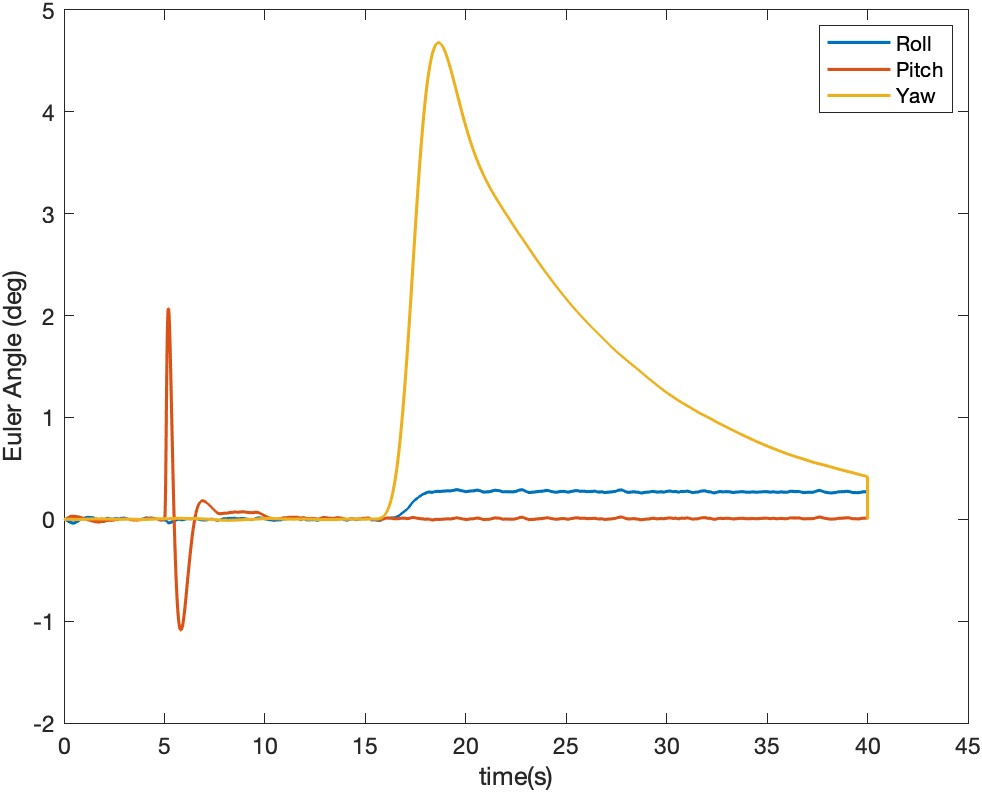
\includegraphics[width=\textwidth]{Images/Gust/VTOL step/4 EulerAngle_5.jpg}
    \caption*{\textit{Euler Angle}}
  \end{minipage}
  \caption{Status of aircraft in multicopter mode when step gust in Y-axis move forward along Y-axis}
  \label{fig:VTOL step yy}
\end{figure}

\subsubsection{Pulse Gust Test for Aircraft in Multi-Copter Mode}

The simulation results for the pulse gust case are comparable to those of the step gust case. Following the occurrence of the gust, the aircraft quickly recovers to a stable hover status. Notably, due to the nature of pulse gusts, aircraft in some instances (as depicted in Figure \ref{fig:VTOL pulse x}) exhibit the ability to withstand larger gusts before experiencing unstable attitudes compared to constant step gusts.

\begin{figure}[htbp]
  \centering
  \begin{minipage}[b]{0.45\textwidth}
    \centering
    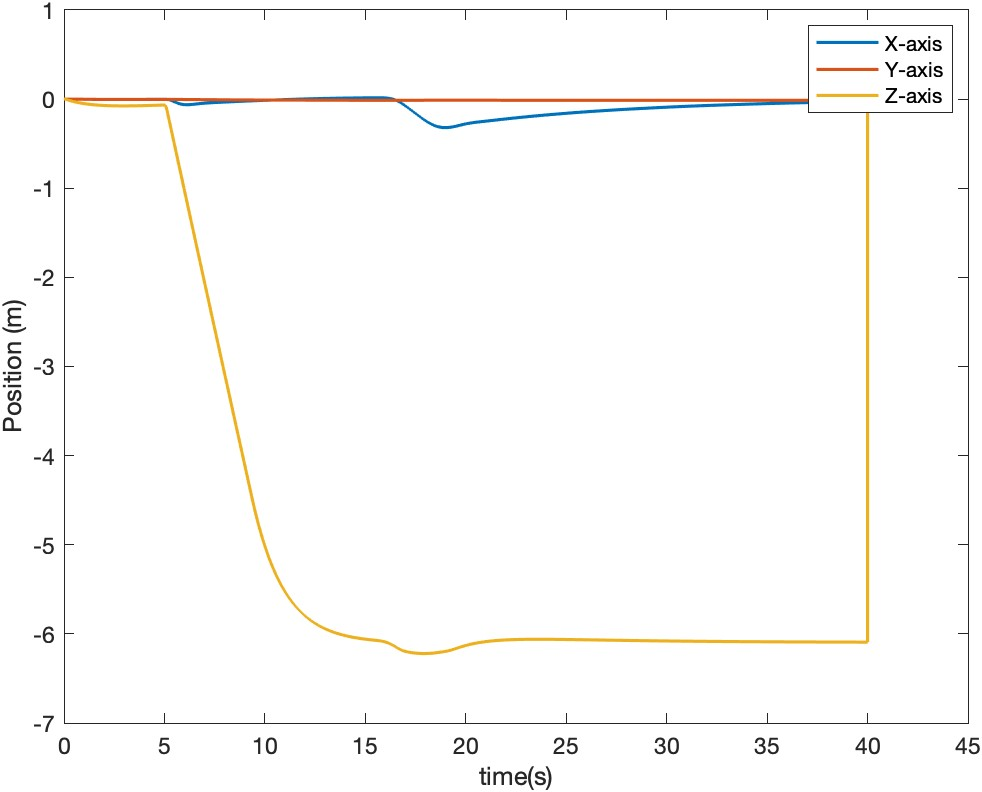
\includegraphics[width=\textwidth]{Images/Gust/VTOL pulse/1 position_1.jpg}
    \caption*{\textit{Position}}
  \end{minipage}
  \hfil
  \begin{minipage}[b]{0.45\textwidth}
    \centering
    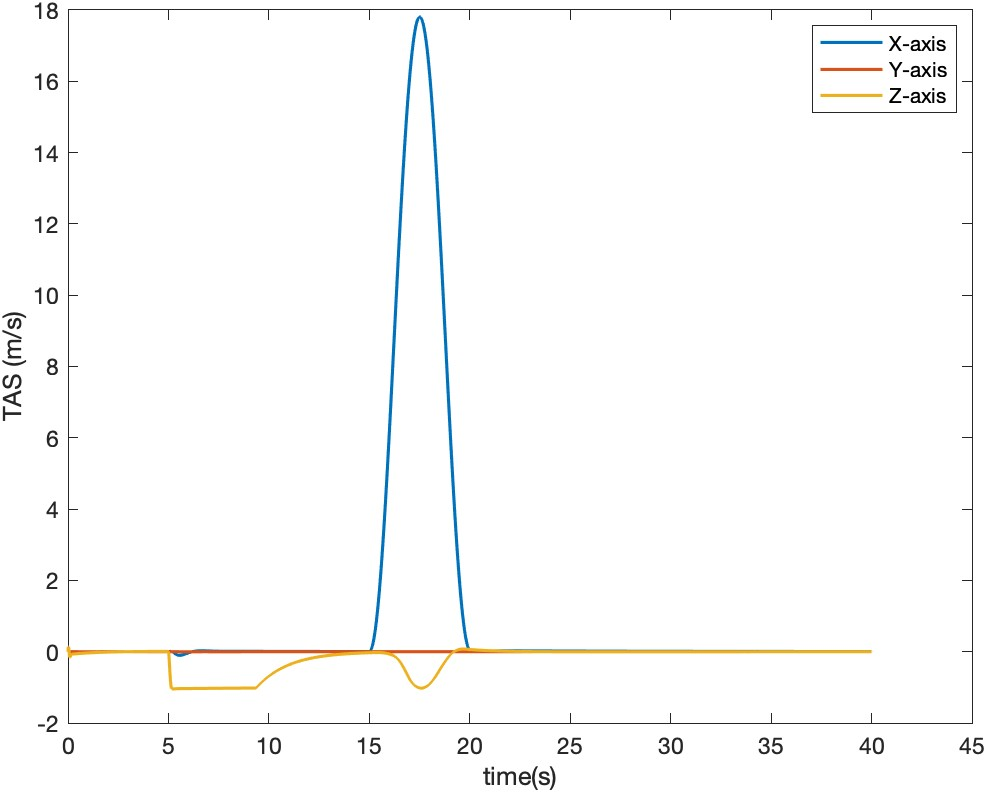
\includegraphics[width=\textwidth]{Images/Gust/VTOL pulse/2 airspeed_1.jpg}
    \caption*{\textit{True Airspeed}}
  \end{minipage}
  \begin{minipage}[b]{0.45\textwidth}
    \centering
    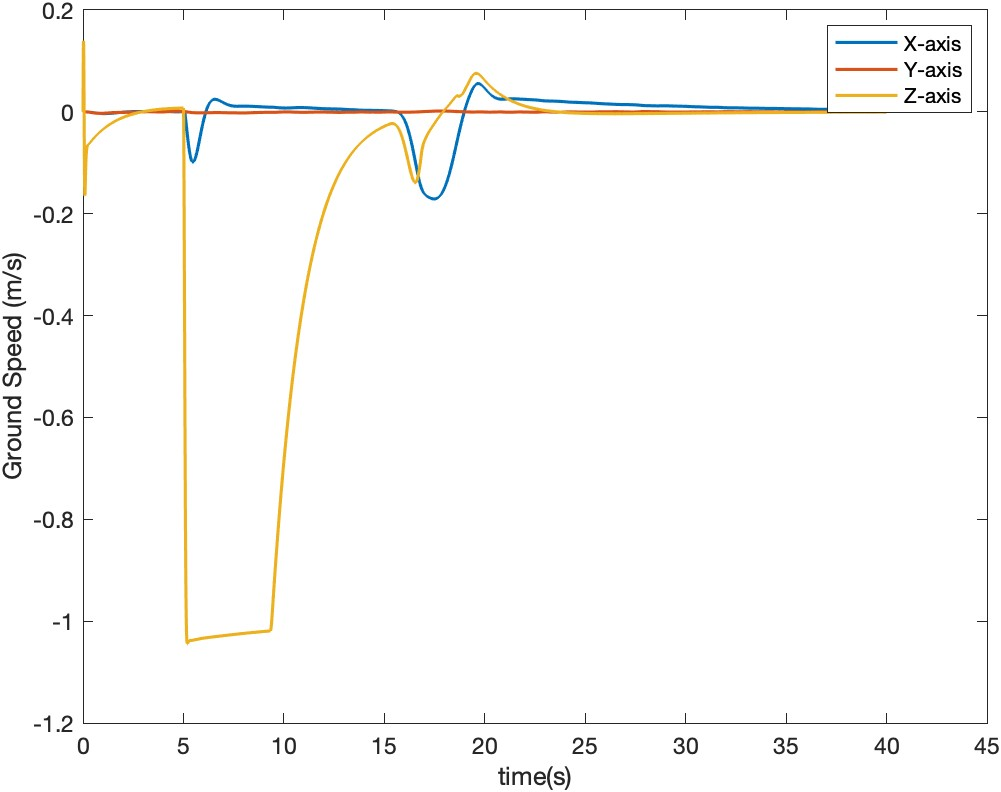
\includegraphics[width=\textwidth]{Images/Gust/VTOL pulse/3 groundspeed_1.jpg}
    \caption*{\textit{Ground Speed}}
  \end{minipage}
  \hfil
  \begin{minipage}[b]{0.45\textwidth}
    \centering
    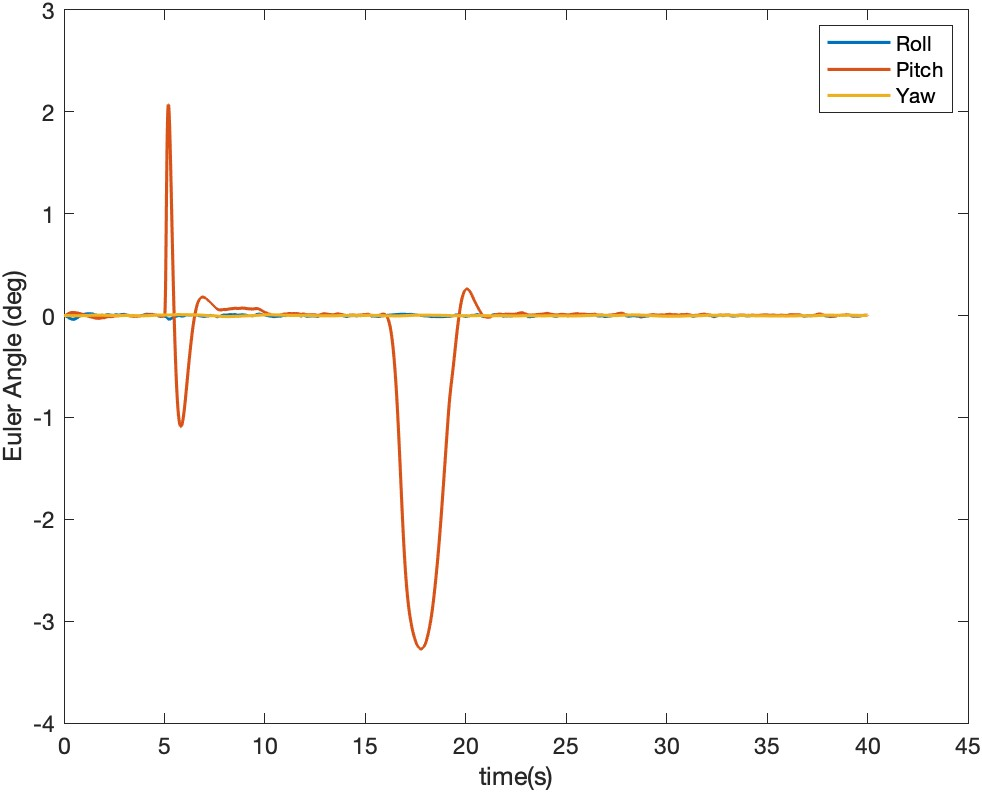
\includegraphics[width=\textwidth]{Images/Gust/VTOL pulse/4 EulerAngle_1.jpg}
    \caption*{\textit{Euler Angle}}
  \end{minipage}
  \caption{Status of aircraft in multicopter mode when pulse gust in negative X-axis move backward along X-axis}
  \label{fig:VTOL pulse -x}
\end{figure}

\begin{figure}[htbp]
  \centering
  \begin{minipage}[b]{0.45\textwidth}
    \centering
    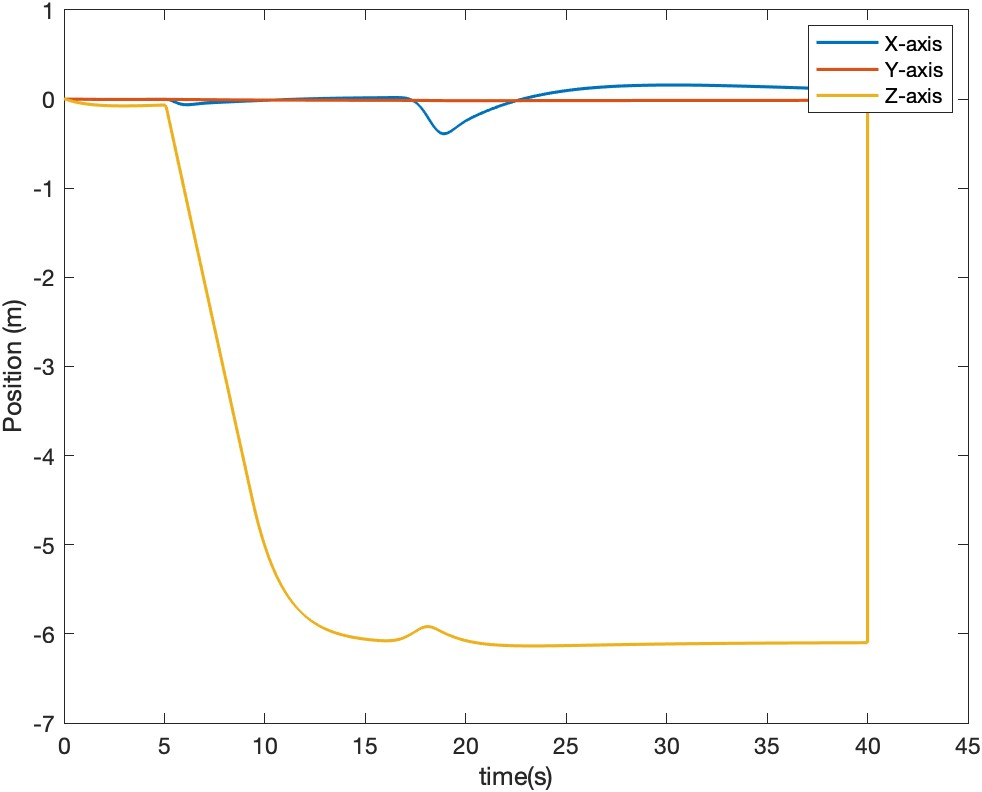
\includegraphics[width=\textwidth]{Images/Gust/VTOL pulse/1 position_2.jpg}
    \caption*{\textit{Position}}
  \end{minipage}
  \hfil
  \begin{minipage}[b]{0.45\textwidth}
    \centering
    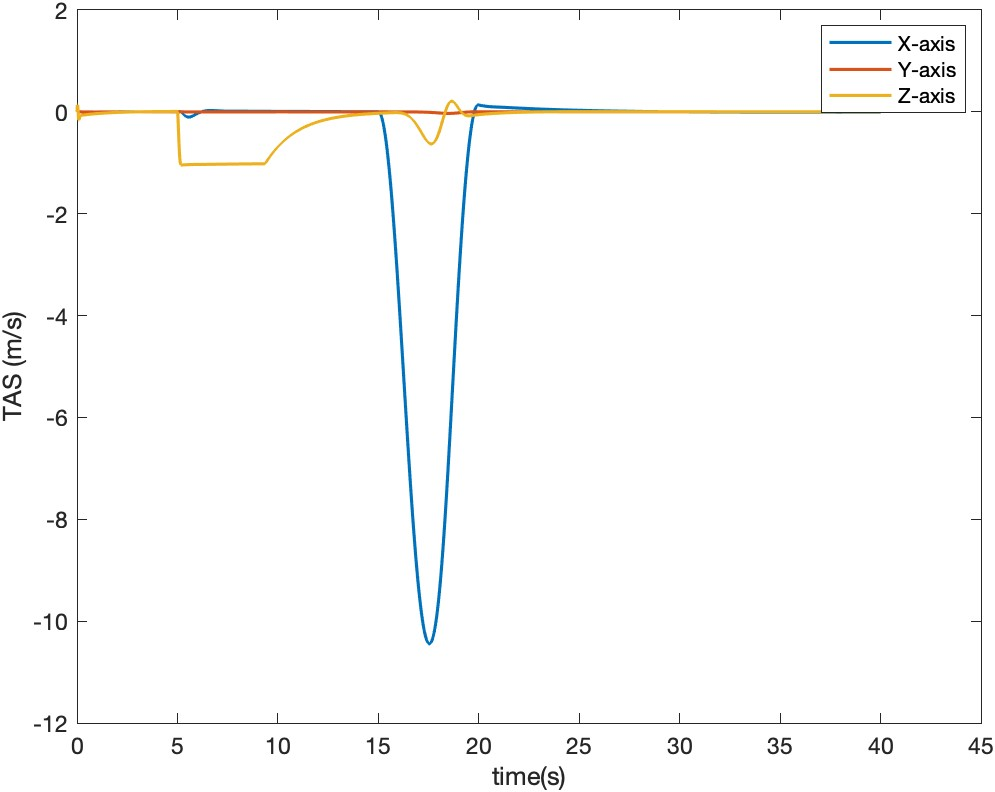
\includegraphics[width=\textwidth]{Images/Gust/VTOL pulse/2 airspeed_2.jpg}
    \caption*{\textit{True Airspeed}}
  \end{minipage}
  \begin{minipage}[b]{0.45\textwidth}
    \centering
    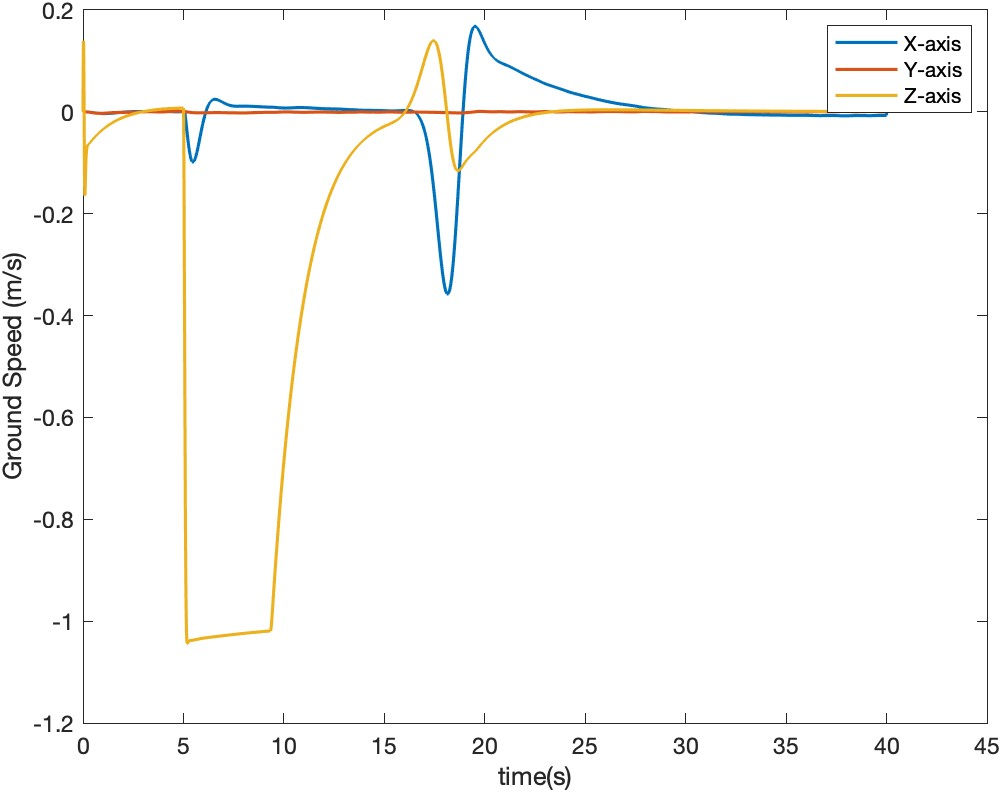
\includegraphics[width=\textwidth]{Images/Gust/VTOL pulse/3 groundspeed_2.jpg}
    \caption*{\textit{Ground Speed}}
  \end{minipage}
  \hfil
  \begin{minipage}[b]{0.45\textwidth}
    \centering
    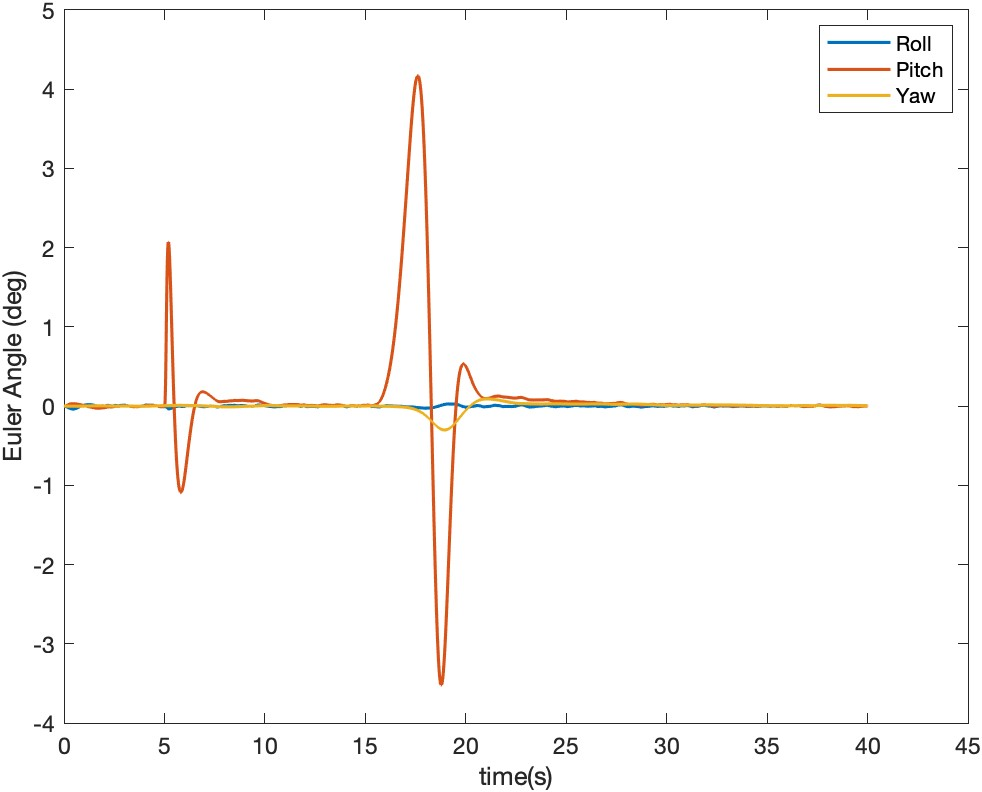
\includegraphics[width=\textwidth]{Images/Gust/VTOL pulse/4 EulerAngle_2.jpg}
    \caption*{\textit{Euler Angle}}
  \end{minipage}
  \caption{Status of aircraft in multicopter mode when pulse gust in positive X-axis move forward along X-axis}
  \label{fig:VTOL pulse x}
\end{figure}

\begin{figure}[htbp]
  \centering
  \begin{minipage}[b]{0.45\textwidth}
    \centering
    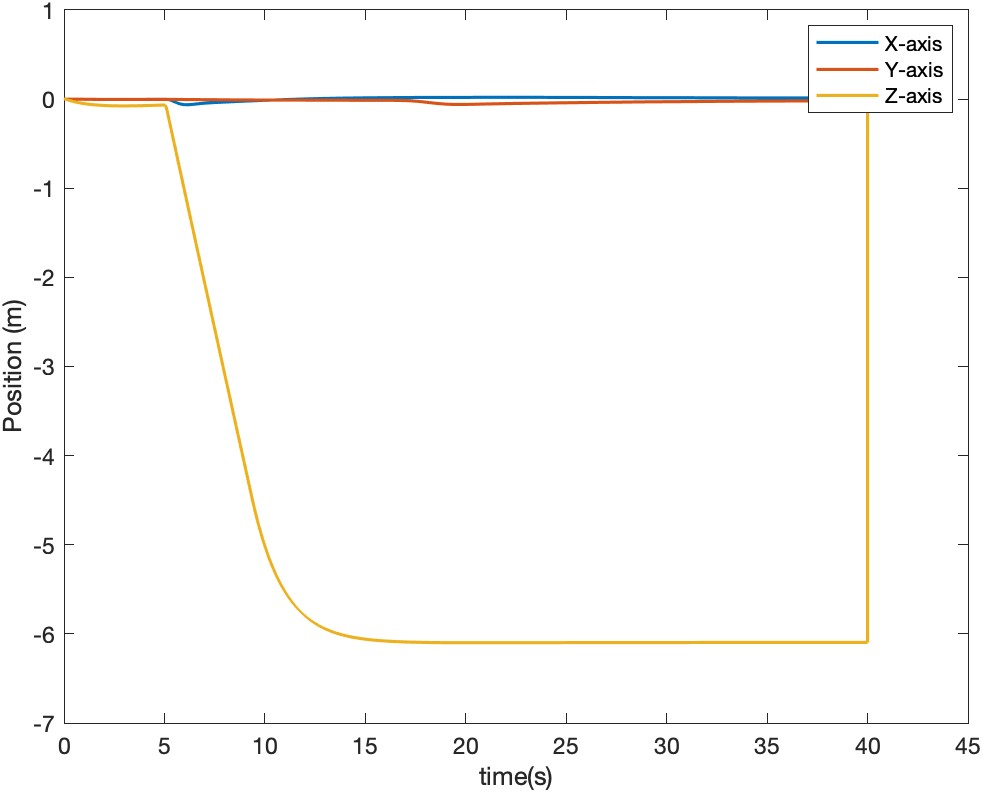
\includegraphics[width=\textwidth]{Images/Gust/VTOL pulse/1 position_3.jpg}
    \caption*{\textit{Position}}
  \end{minipage}
  \hfil
  \begin{minipage}[b]{0.45\textwidth}
    \centering
    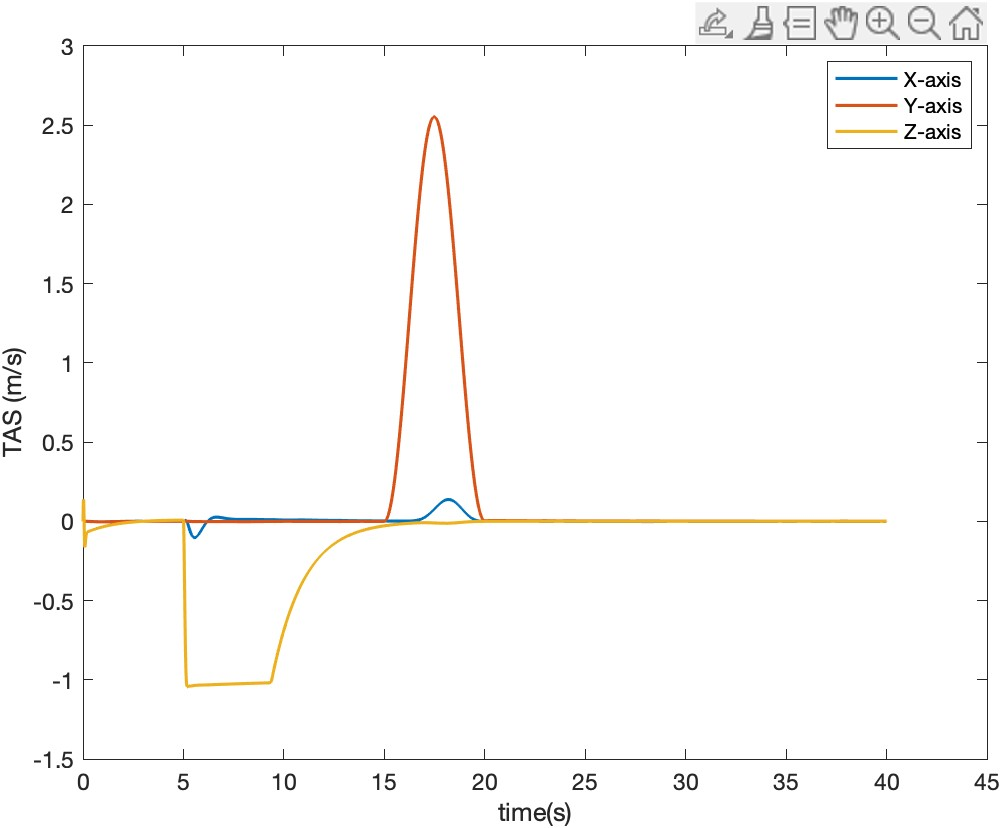
\includegraphics[width=\textwidth]{Images/Gust/VTOL pulse/2 airspeed_3.jpg}
    \caption*{\textit{True Airspeed}}
  \end{minipage}
  \begin{minipage}[b]{0.45\textwidth}
    \centering
    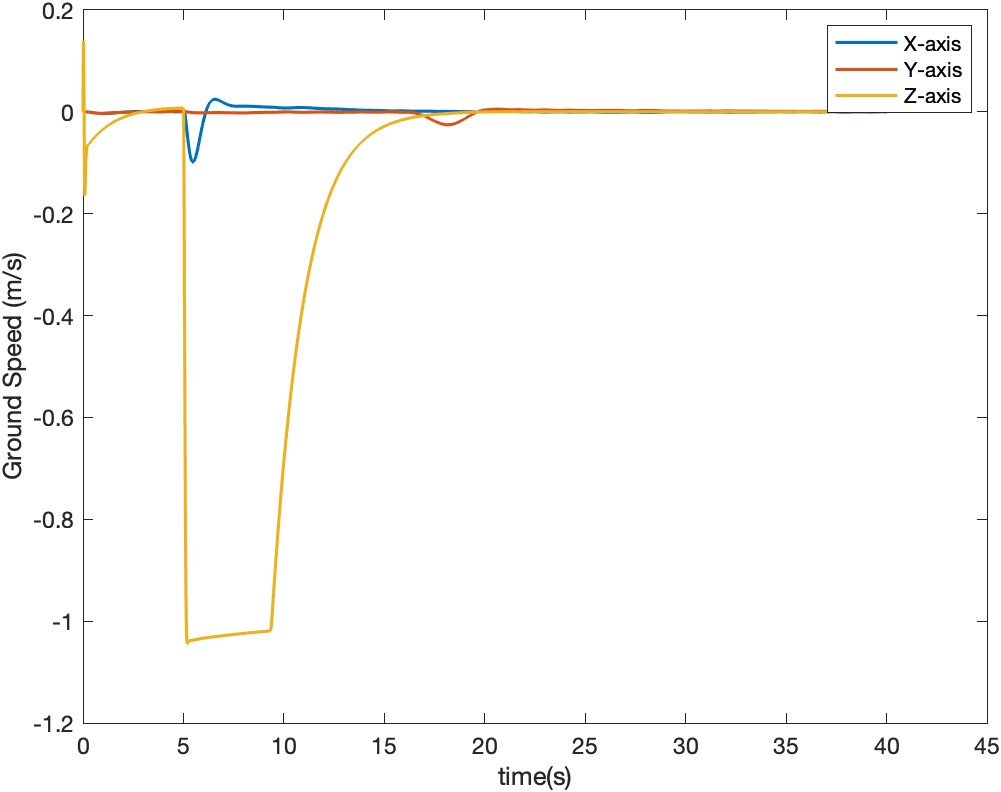
\includegraphics[width=\textwidth]{Images/Gust/VTOL pulse/3 groundspeed_3.jpg}
    \caption*{\textit{Ground Speed}}
  \end{minipage}
  \hfil
  \begin{minipage}[b]{0.45\textwidth}
    \centering
    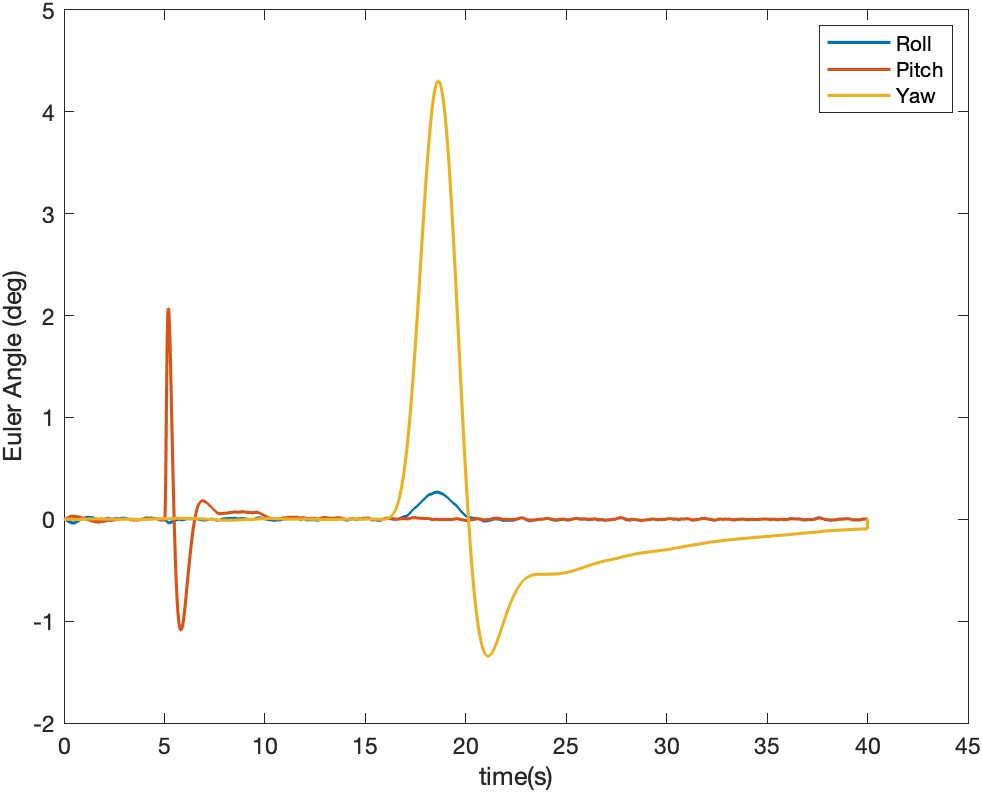
\includegraphics[width=\textwidth]{Images/Gust/VTOL pulse/4 EulerAngle_3.jpg}
    \caption*{\textit{Euler Angle}}
  \end{minipage}
  \caption{Status in aircraft in multicopter mode when pulse gust in Y-axis move backward along X-axis}
  \label{fig:VTOL pulse xy}
\end{figure}

\begin{figure}[htbp]
  \centering
  \begin{minipage}[b]{0.45\textwidth}
    \centering
    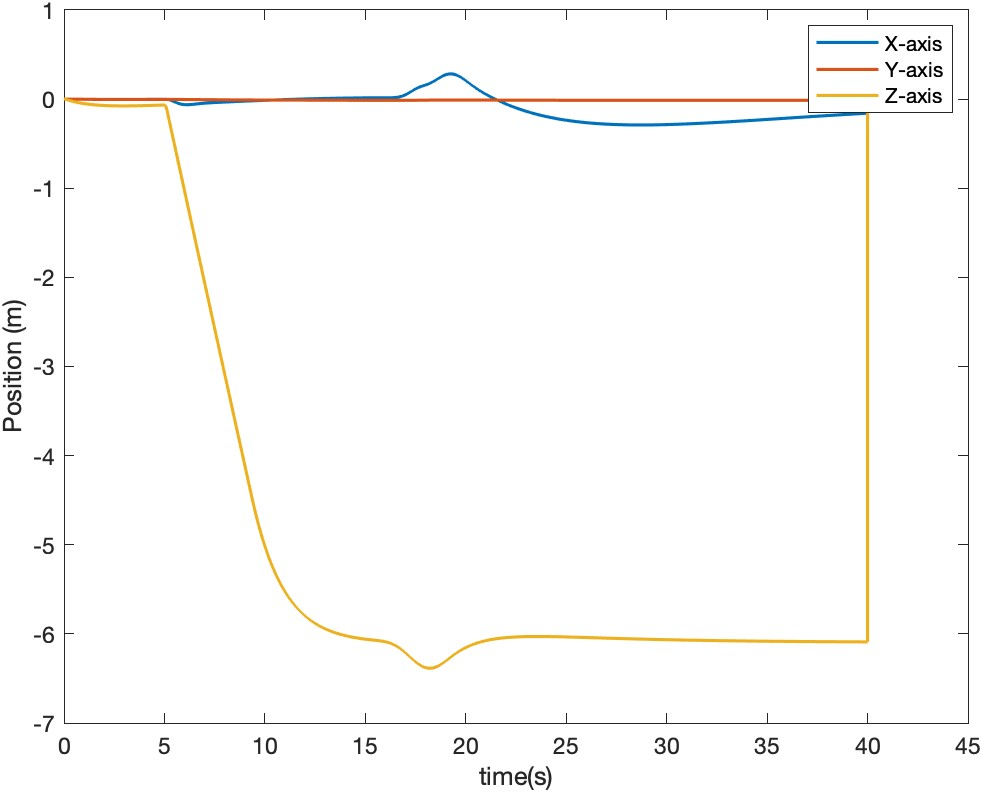
\includegraphics[width=\textwidth]{Images/Gust/VTOL pulse/1 position_4.jpg}
    \caption*{\textit{Position}}
  \end{minipage}
  \hfil
  \begin{minipage}[b]{0.45\textwidth}
    \centering
    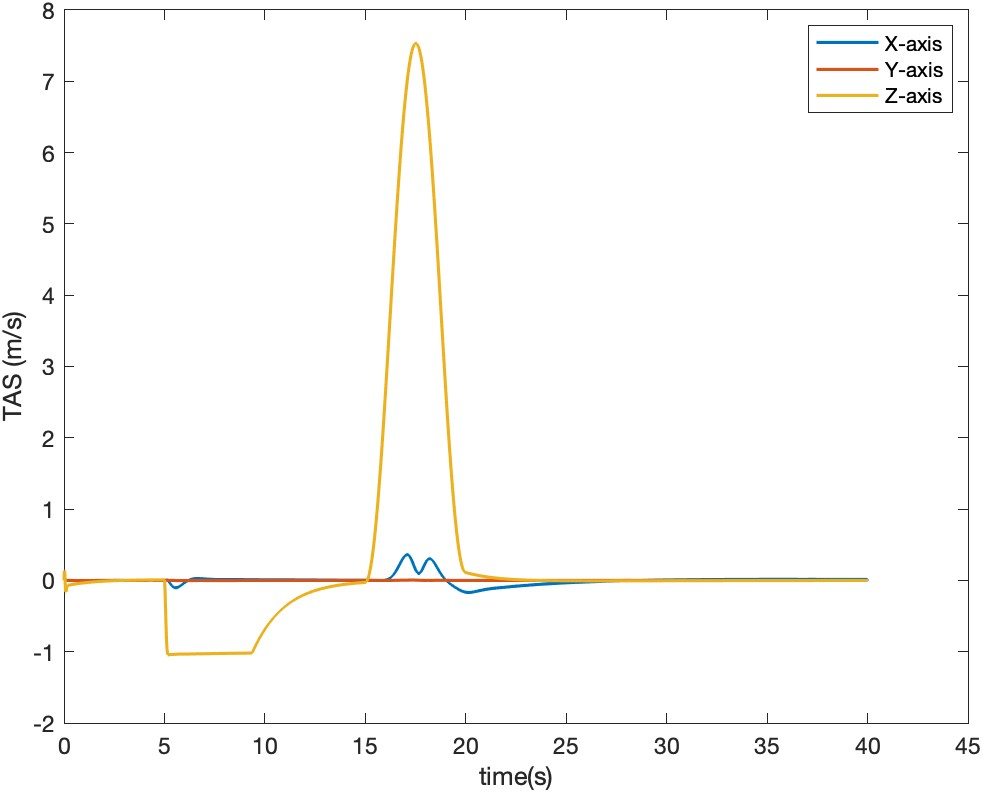
\includegraphics[width=\textwidth]{Images/Gust/VTOL pulse/2 airspeed_4.jpg}
    \caption*{\textit{True Airspeed}}
  \end{minipage}
  \begin{minipage}[b]{0.45\textwidth}
    \centering
    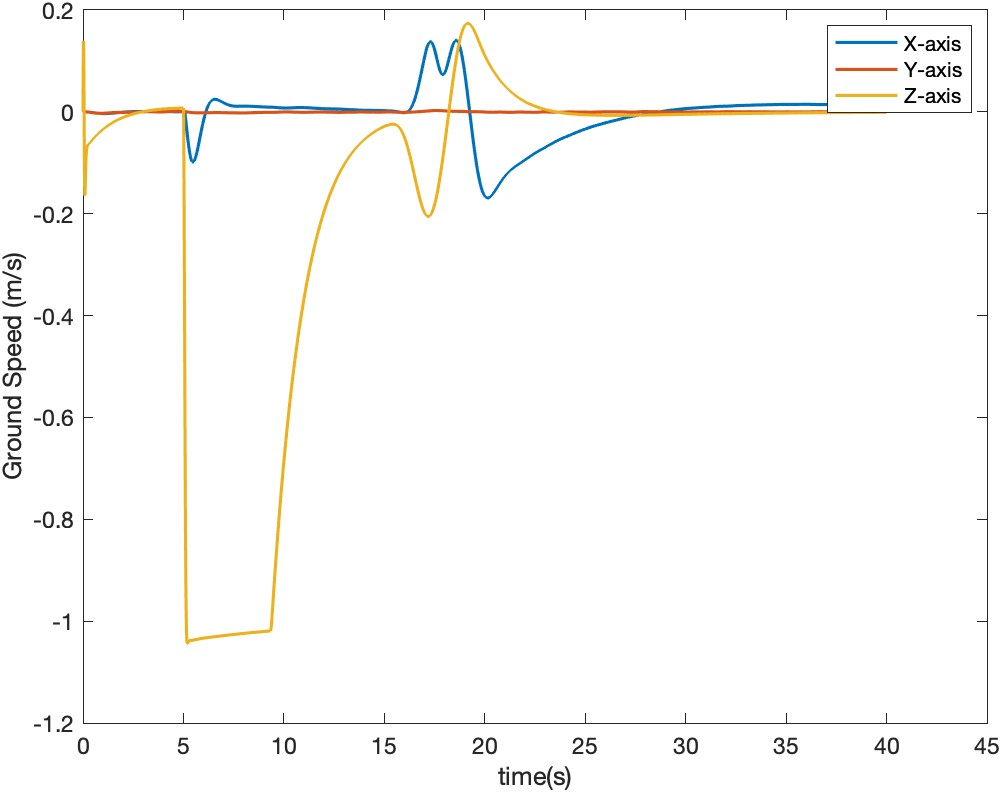
\includegraphics[width=\textwidth]{Images/Gust/VTOL pulse/3 groundspeed_4.jpg}
    \caption*{\textit{Ground Speed}}
  \end{minipage}
  \hfil
  \begin{minipage}[b]{0.45\textwidth}
    \centering
    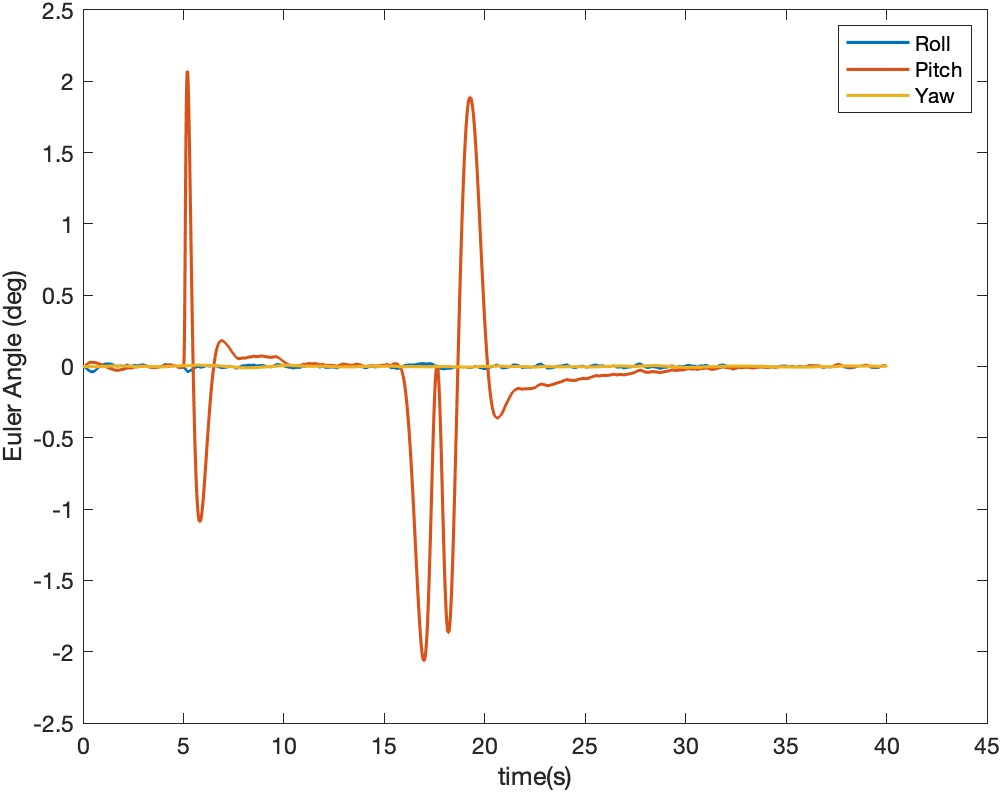
\includegraphics[width=\textwidth]{Images/Gust/VTOL pulse/4 EulerAngle_4.jpg}
    \caption*{\textit{Euler Angle}}
  \end{minipage}
  \caption{Status of aircraft in multicopter mode when pulse gust in Z-axis move backward along X-axis}
  \label{fig:VTOL pulse z}
\end{figure}

\begin{figure}[htbp]
  \centering
  \begin{minipage}[b]{0.45\textwidth}
    \centering
    \includegraphics[width=\textwidth]{Images/Gust/VTOL pulse/1 position_5.jpg}
    \caption*{\textit{Position}}
  \end{minipage}
  \hfil
  \begin{minipage}[b]{0.45\textwidth}
    \centering
    \includegraphics[width=\textwidth]{Images/Gust/VTOL pulse/2 airspeed_5.jpg}
    \caption*{\textit{True Airspeed}}
  \end{minipage}
  \begin{minipage}[b]{0.45\textwidth}
    \centering
    \includegraphics[width=\textwidth]{Images/Gust/VTOL pulse/3 groundspeed_5.jpg}
    \caption*{\textit{Ground Speed}}
  \end{minipage}
  \hfil
  \begin{minipage}[b]{0.45\textwidth}
    \centering
    \includegraphics[width=\textwidth]{Images/Gust/VTOL pulse/4 EulerAngle_5.jpg}
    \caption*{\textit{Euler Angle}}
  \end{minipage}
  \caption{Status of aircraft in multicopter mode when pulse gust in Y-axis move forward along Y-axis}
  \label{fig:VTOL pulse yy}
\end{figure}

\subsubsection{Pulse Gust Test in Forward Flight Mode}

During the Pulse Gust Test in forward flight mode, the control system transitions to fixed-wing mode, maintaining constant $v_{\text{cruise}}$ and altitude. Yaw and roll angle control are set to null.

The incorporation of an additional saturation module into the pitch setpoint input of the $TECS_m$ control system facilitated the examination of pulse gusty wind effects in forward flight mode. Unlike step gusts, which are unrealistic in forward flight mode, only pulse gusty winds were considered. Key observations from these conditions are detailed below:

At approximately 10 seconds into the simulation, the drone encountered a pulse gust of wind. Due to the concurrent movement of the aircraft and gusty wind along the X-axis, precise synchronization between the gust and the drone's position was unattainable. Consequently, the aircraft could only withstand gusts of up to 5 knots from the X direction without compromising its stability. In other scenarios, the aircraft demonstrated resilience against pulse gusts of up to 15 knots.

In Figure \ref{fig:Gust FWD pulse y}, the simulation results indicate an additional yaw angle generated after a gust in the Y-axis occurs, causing the aircraft to deviate from its original course.

When subjected to a pulse gust along the Z-axis, control complexity increased due to changes in altitude and airspeed. Figure \ref{fig:Gust FWD pulse z} illustrates the response of the $TECS_m$ system, tasked with maintaining airspeed while controlling altitude to return to the designated altitude. This simultaneous adjustment of throttle and movable surfaces introduced delays, particularly evident in altitude control due to the high value of the integration factor in the $TECS_m$ system. Consequently, the total control system required additional time to stabilize the aircraft.

\begin{figure}[htbp]
  \centering
  \begin{minipage}[b]{0.45\textwidth}
    \centering
    \includegraphics[width=\textwidth]{Images/Gust/Gust FWD pulse 0428/1 position_1.jpg}
    \caption*{\textit{Position}}
  \end{minipage}
  \hfil
  \begin{minipage}[b]{0.45\textwidth}
    \centering
    \includegraphics[width=\textwidth]{Images/Gust/Gust FWD pulse 0428/2 TAS_1.jpg}
    \caption*{\textit{Airspeed in global frame}}
  \end{minipage}
  \begin{minipage}[b]{0.45\textwidth}
    \centering
    \includegraphics[width=\textwidth]{Images/Gust/Gust FWD pulse 0428/3 groundspeed_1.jpg}
    \caption*{\textit{Ground Speed}}
  \end{minipage}
  \hfil
  \begin{minipage}[b]{0.45\textwidth}
    \centering
    \includegraphics[width=\textwidth]{Images/Gust/Gust FWD pulse 0428/4 EulerAngle_1.jpg}
    \caption*{\textit{Euler Angle}}
  \end{minipage}
  \begin{minipage}[b]{0.45\textwidth}
    \centering
    \includegraphics[width=\textwidth]{Images/Gust/Gust FWD pulse 0428/5 Throttle_1.jpg}
    \caption*{\textit{Throttle}}
  \end{minipage}
  \hfil
  \begin{minipage}[b]{0.45\textwidth}
    \centering
    \includegraphics[width=\textwidth]{Images/Gust/Gust FWD pulse 0428/6 Airspeed_1.jpg}
    \caption*{\textit{Airspeed}}
  \end{minipage}
  \caption{Status of aircraft in fixed-wing mode when pulse gust in X-axis move backward along X-axis}
  \label{fig:Gust FWD pulse -x}
\end{figure}

\begin{figure}[htbp]
  \centering
  \begin{minipage}[b]{0.45\textwidth}
    \centering
    \includegraphics[width=\textwidth]{Images/Gust/Gust FWD pulse 0428/1 position_2.jpg}
    \caption*{\textit{Position}}
  \end{minipage}
  \hfil
  \begin{minipage}[b]{0.45\textwidth}
    \centering
    \includegraphics[width=\textwidth]{Images/Gust/Gust FWD pulse 0428/2 TAS_2.jpg}
    \caption*{\textit{Airspeed in global frame}}
  \end{minipage}
  \begin{minipage}[b]{0.45\textwidth}
    \centering
    \includegraphics[width=\textwidth]{Images/Gust/Gust FWD pulse 0428/3 groundspeed_2.jpg}
    \caption*{\textit{Ground Speed}}
  \end{minipage}
  \hfil
  \begin{minipage}[b]{0.45\textwidth}
    \centering
    \includegraphics[width=\textwidth]{Images/Gust/Gust FWD pulse 0428/4 EulerAngle_2.jpg}
    \caption*{\textit{Euler Angle}}
  \end{minipage}
  \begin{minipage}[b]{0.45\textwidth}
    \centering
    \includegraphics[width=\textwidth]{Images/Gust/Gust FWD pulse 0428/5 Throttle_2.jpg}
    \caption*{\textit{Throttle}}
  \end{minipage}
  \hfil
  \begin{minipage}[b]{0.45\textwidth}
    \centering
    \includegraphics[width=\textwidth]{Images/Gust/Gust FWD pulse 0428/6 Airspeed_2.jpg}
    \caption*{\textit{Airspeed}}
  \end{minipage}
  \caption{Status of aircraft in fixed-wing mode when pulse gust in X-axis move backward along X-axis}
  \label{fig:Gust FWD pulse x}
\end{figure}

\begin{figure}[htbp]
  \centering
  \begin{minipage}[b]{0.45\textwidth}
    \centering
    \includegraphics[width=\textwidth]{Images/Gust/Gust FWD pulse 0428/1 position_3.jpg}
    \caption*{\textit{Position}}
  \end{minipage}
  \hfil
  \begin{minipage}[b]{0.45\textwidth}
    \centering
    \includegraphics[width=\textwidth]{Images/Gust/Gust FWD pulse 0428/2 TAS_3.jpg}
    \caption*{\textit{Airspeed in global frame}}
  \end{minipage}
  \begin{minipage}[b]{0.45\textwidth}
    \centering
    \includegraphics[width=\textwidth]{Images/Gust/Gust FWD pulse 0428/3 groundspeed_3.jpg}
    \caption*{\textit{Ground Speed}}
  \end{minipage}
  \hfil
  \begin{minipage}[b]{0.45\textwidth}
    \centering
    \includegraphics[width=\textwidth]{Images/Gust/Gust FWD pulse 0428/4 EulerAngle_3.jpg}
    \caption*{\textit{Euler Angle}}
  \end{minipage}
  \begin{minipage}[b]{0.45\textwidth}
    \centering
    \includegraphics[width=\textwidth]{Images/Gust/Gust FWD pulse 0428/5 Throttle_3.jpg}
    \caption*{\textit{Throttle}}
  \end{minipage}
  \hfil
  \begin{minipage}[b]{0.45\textwidth}
    \centering
    \includegraphics[width=\textwidth]{Images/Gust/Gust FWD pulse 0428/6 Airspeed_3.jpg}
    \caption*{\textit{Airspeed}}
  \end{minipage}
  \caption{Status of aircraft in fixed-wing mode when pulse gust in Y-axis move backward along X-axis}
  \label{fig:Gust FWD pulse y}
\end{figure}

\begin{figure}[htbp]
  \centering
  \begin{minipage}[b]{0.45\textwidth}
    \centering
    \includegraphics[width=\textwidth]{Images/Gust/Gust FWD pulse 0428/1 position_4.jpg}
    \caption*{\textit{Position}}
  \end{minipage}
  \hfil
  \begin{minipage}[b]{0.45\textwidth}
    \centering
    \includegraphics[width=\textwidth]{Images/Gust/Gust FWD pulse 0428/2 TAS_4.jpg}
    \caption*{\textit{Airspeed in global frame}}
  \end{minipage}
  \begin{minipage}[b]{0.45\textwidth}
    \centering
    \includegraphics[width=\textwidth]{Images/Gust/Gust FWD pulse 0428/3 groundspeed_4.jpg}
    \caption*{\textit{Ground Speed}}
  \end{minipage}
  \hfil
  \begin{minipage}[b]{0.45\textwidth}
    \centering
    \includegraphics[width=\textwidth]{Images/Gust/Gust FWD pulse 0428/4 EulerAngle_4.jpg}
    \caption*{\textit{Euler Angle}}
  \end{minipage}
  \begin{minipage}[b]{0.45\textwidth}
    \centering
    \includegraphics[width=\textwidth]{Images/Gust/Gust FWD pulse 0428/5 Throttle_4.jpg}
    \caption*{\textit{Throttle}}
  \end{minipage}
  \hfil
  \begin{minipage}[b]{0.45\textwidth}
    \centering
    \includegraphics[width=\textwidth]{Images/Gust/Gust FWD pulse 0428/6 Airspeed_4.jpg}
    \caption*{\textit{Airspeed}}
  \end{minipage}
  \caption{Status of aircraft in fixed-wing mode when pulse gust in Z-axis move backward along X-axis}
  \label{fig:Gust FWD pulse z}
\end{figure}

\subsubsection{High-Frequency Oscillation Analysis of Elevator Control}

During the Gust in Z-axis test in forward flight mode, a high-frequency oscillation of the elevator control was observed. Upon comparing each input signal to the attitude control block in the forward (FWD) control system, which includes attitude error and angular velocity error, it was identified that the distribution of the input signal primarily stems from two components: the error between the required pitch angle and the current pitch angle (Pitch Error in Figure \ref{fig:Control Surface Analysis 2}), and the error of angular velocity in the pitch angle part (angular velocity in Figure \ref{fig:Control Surface Analysis 2}). Upon comparison of the values and parameter values, it was determined that the latter component mainly contributes to the high-frequency oscillation of the elevator command signal, aimed at counteracting the angular velocity. Due to the hardware response delay effect, the actual change in elevator angle value is smoother than the command signal from the control system (Control Surface in Figure \ref{fig:Control Surface Analysis 2}).

\begin{figure}[htbp]
  \centering
  \begin{minipage}[b]{0.45\textwidth}
    \centering
    \includegraphics[width=\textwidth]{Images/Control Surface Analysis/1 position_1.jpg}
    \caption*{\textit{Position}}
  \end{minipage}
  \hfil
  \begin{minipage}[b]{0.45\textwidth}
    \centering
    \includegraphics[width=\textwidth]{Images/Control Surface Analysis/2 TAS_1.jpg}
    \caption*{\textit{Airspeed}}
  \end{minipage}
  \begin{minipage}[b]{0.45\textwidth}
    \centering
    \includegraphics[width=\textwidth]{Images/Control Surface Analysis/3 groundspeed_1.jpg}
    \caption*{\textit{Ground Speed}}
  \end{minipage}
  \hfil
  \begin{minipage}[b]{0.45\textwidth}
    \centering
    \includegraphics[width=\textwidth]{Images/Control Surface Analysis/5 Throttle_1.jpg}
    \caption*{\textit{Throttle}}
  \end{minipage}
  \caption{Status of aircraft in fixed-wing mode when pulse gust in Z-axis move backward along X-axis (a)}
  \label{fig:Control Surface Analysis 1}
\end{figure}

\begin{figure}[htbp]
  \centering
  \begin{minipage}[b]{0.45\textwidth}
    \centering
    \includegraphics[width=\textwidth]{Images/Control Surface Analysis/4 EulerAngle_1.jpg}
    \caption*{\textit{Euler Angle}}
  \end{minipage}
  \hfil
  \begin{minipage}[b]{0.45\textwidth}
    \centering
    \includegraphics[width=\textwidth]{Images/Control Surface Analysis/6 EulerAngleVelocity_1.jpg}
    \caption*{\textit{Angular Velocity}}
  \end{minipage}
  \begin{minipage}[b]{0.45\textwidth}
    \centering
    \includegraphics[width=\textwidth]{Images/Control Surface Analysis/7 PitchEror_1.jpg}
    \caption*{\textit{Pitch Error}}
  \end{minipage}
  \hfil
  \begin{minipage}[b]{0.45\textwidth}
    \centering
    \includegraphics[width=\textwidth]{Images/Control Surface Analysis/8 ControlSurface_1.jpg}
    \caption*{\textit{Control Surface}}
  \end{minipage}
  \caption{Status of aircraft in fixed-wing mode when pulse gust in Z-axis move backward along X-axis (b)}
  \label{fig:Control Surface Analysis 2}
\end{figure}

\section{Transition Controller}
\label{section:Transition Strategy}

The transition control strategy draws from the comprehensive study conducted by \cite{battaini2022}. In their work, the transient process from multi-copter mode to fixed-wing mode has been thoroughly analyzed and realized. However, the back transition strategy, facilitating the shift from fixed-wing mode back to multi-copter mode, was formulated but not subjected to simulation in their study. This paper aims to extend the prior research by re-evaluating the transition process from multi-copter mode to fixed-wing mode and completing the back transition simulation.

\subsection{Transition Strategy}

The transition from multi-copter mode to fixed-wing mode is achieved by accelerating forward; as the speed increases, the wings start producing lift that gradually replaces the vertical force produced by the vertical motors to ensure equilibrium in the longitudinal plane. In  \cite{battaini2022}, the $TECS_m$ control has been compared, showing superior performance. In this simulation, the control system selects $TECS_m$ as the fixed-wing mode directly, and the strategy is described by the following steps:

\begin{enumerate}
    \item Hovering condition: null airspeed, level attitude. Multicopter control ON (in POSITION MODE).
    \item Transition switch is activated.
    \item Multicopter control switches to ALTITUDE MODE.
    \item The fixed-wing controller is turned ON (in ALTITUDE) with a velocity setpoint of $15 \, \text{m/s}$. Forward motors are activated at full throttle and the VTOL starts to accelerate.
    \item Level attitude setpoint is maintained both from vertical motors and control surfaces, splitting the required control effort among the two controllers.
    \item Airspeed and lift increase; at the same time multicopter vertical force decreases.
    \item Once the stall speed is reached, the fixed-wing controller takes full control. Multicopter control is turned OFF since the weight of the VTOL is fully balanced by the lift. Attitude (pitch setpoint) now is managed by TECS.
    \item The VTOL continues to accelerate up to $v_{\text{cruise}}$.
    \item Transition is completed.
\end{enumerate}

In particular, the following actions are needed in order to correctly mix the contribution of the controllers during the transition phase:

\begin{itemize}
    \item The command surfaces deflections are weighted as functions of airspeed with the scaling factor $K_{\text{FW}}$ (figure \ref{fig:Scaling factors}), that is defined as:
    \begin{equation}
        K_{\text{FW}} = \frac{V}{V_{\text{stall}}}
    \end{equation}
    and limited between $0$ and $1$. So, the control surfaces have reduced authority at low speed and full authority at speeds above the stall speed.
    
    \item The multicopter control moments are weighted as functions of airspeed with the scaling factor $K_{\text{MC}}$ (figure \ref{fig:Scaling factors}), that is defined as:
    \begin{equation}
        K_{\text{MC}} = 1 - \frac{V}{V_{\text{stall}}}
    \end{equation}
    and limited between $0$ and $1$. So, the multicopter controller has full authority at low speed, which decreases with the increase of speed. Above the stall speed, it is turned off.
    
    \item Instead of ignoring the pitch setpoint calculated by TECS, the energy balance rate $\dot{L}_e$ is set to zero for airspeed smaller than the stall speed: the TECS algorithm returns a null pitch angle. When the stall speed is reached, this quantity returns to its real value, and the pitch setpoint necessary to fly in fixed-wing mode in that condition is calculated. This is done by the scaling factor $K_{\text{PITCH}}$ (figure \ref{fig:Scaling factors}). The value does not go instantly to one but starts rising just before the stall speed.
\end{itemize}

\begin{figure}
    \centering
    \includegraphics[width=0.85\linewidth]{Images/Scaling factors.png}
    \caption{Scaling factors.}
    \label{fig:Scaling factors}
\end{figure}

\subsection{Back Transition Strategy}
\label{section:Back Transition Strategy}
Back transition is the inverse process with respect to transition: the aircraft goes from a fixed-wing condition to hovering condition in multicopter mode. This must be achieved without altitude loss and in the shortest time and distance. A possible strategy, which is not yet simulated, can be:
\begin{itemize}
    \item Starting point: fixed-wing mode at any airspeed.
    \item Back transition switch is activated.
    \item The airspeed is reduced by setting the throttle to idle and using air brakes. Height is maintained with the elevator action; the VTOL will be pitched up.
    \item Once the stall speed is reached, the multicopter controller is turned ON while the fixed-wing controller is turned OFF.
    \item Ending point: hovering condition.
\end{itemize}

The activation of the multicopter controller in POSITION MODE can cause abrupt maneuvers; the option to use only the velocity loop with null speed setpoint might be considered. Once stopped, POSITION MODE is enabled in order to maintain the current position.

\subsection{Simulation}
The simulation results depicted in Figure \ref{fig:TRANS mission} illustrate the transient phase, comprising both the transition and back transition phases. Following a vertical take-off and climb mission, the aircraft, under multicopter mode control, ascends to the desired altitude and stabilizes in a hover state. At 30 seconds into the simulation, the transition phase commences, as detailed in Section \ref{section:Transition Strategy}. During this phase, the horizontal propeller is engaged to accelerate the drone to an airspeed of 14 m/s, while simultaneously reducing the vertical propeller thrust. Upon achieving the target airspeed of 14 m/s, the multicopter mode is deactivated, and full fixed-wing mode control is engaged, continuing the acceleration to reach 15 m/s.

At 80 seconds, the aircraft enters the back transition phase, described in Section \ref{section:Back Transition Strategy}. Using movable surfaces, the aircraft decelerates to below 14 m/s, and at 86.5 seconds into the simulation, the flight speed reaches 14 m/s. At this point, the fixed-wing mode is deactivated, and the multicopter mode is activated to assume full control of the drone. Subsequently, from 86.5 seconds onward, the drone decelerates back to a hover status under full multicopter mode control. 

The back transition strategy outlined in \cite{battaini2022} involves setting the rate control to null velocity setpoint, leading to abrupt maneuvers in pitch angle during the transition from fixed-wing mode to multicopter mode. As an alternative approach, a more conservative strategy is adopted in the simulation. In this strategy, when the control system switches to multicopter mode, the rate control employs a constant deceleration value of $0.25 
 m/s^2$, ensuring a smooth transition from fixed-wing control to multicopter control.

\begin{figure}[htbp]
  \centering
  \begin{minipage}[b]{0.45\textwidth}
    \centering
    \includegraphics[width=\textwidth]{Images/TRANS/1 position_1.jpg}
    \caption*{\textit{Position}}
  \end{minipage}
  \hfil
  \begin{minipage}[b]{0.45\textwidth}
    \centering
    \includegraphics[width=\textwidth]{Images/TRANS/2 TAS_1.jpg}
    \caption*{\textit{Airspeed}}
  \end{minipage}
  \begin{minipage}[b]{0.45\textwidth}
    \centering
    \includegraphics[width=\textwidth]{Images/TRANS/3 EulerAngle_1.jpg}
    \caption*{\textit{Euler Angle}}
  \end{minipage}
  \hfil
  \begin{minipage}[b]{0.45\textwidth}
    \centering
    \includegraphics[width=\textwidth]{Images/TRANS/4 MovableSurface_1.jpg}
    \caption*{\textit{Movable Surface Control}}
  \end{minipage}
  \begin{minipage}[b]{0.45\textwidth}
    \centering
    \includegraphics[width=\textwidth]{Images/TRANS/5 Throttle_1.jpg}
    \caption*{\textit{Throttle}}
  \end{minipage}
  \hfil
  \begin{minipage}[b]{0.45\textwidth}
    \centering
    \includegraphics[width=\textwidth]{Images/TRANS/6 FlightMode_1.jpg}
    \caption*{\textit{Flight Mode}}
  \end{minipage}
  \caption{Status in mission including transition and back transition}
  \label{fig:TRANS mission}
\end{figure}

\subsection{Evaluation}

Figure \ref{fig:TRANS mission} illustrates the transition phase, which exhibits a 3-meter height loss and a slight velocity overshoot of 0.25 m/s. This occurrence results from the abrupt acceleration in fixed-wing control and the proportional throttle reduction in multi-copter control. At approximately 52.4 seconds into the simulation, abrupt changes in throttle for both horizontal and vertical motors are observed. This abrupt change is attributed to the sudden activation of pitch angle control in fixed-wing mode by $K_{pitch}$, prompted by the increase in airspeed from 12 m/s to 13 m/s during this period. Additionally, analysis of Euler angles and movable surface controls in Figure \ref{fig:TRANS mission} reveals significant pitch angle oscillations during the transition. These oscillations are crucial for balancing force distribution, facilitating the switch to fixed-wing mode.

During the transition phase, the switch from multi-copter mode to fixed-wing mode induces an additional yaw angle, resulting in a 60-meter movement along the Y-axis during the forward flight phase. In the back transition phase, as an alternative strategy, proportional reductions in velocity along the X-axis and Y-axis could be employed to mitigate abrupt control changes. Yaw angle control would be implemented after the aircraft returns to hover status.

In the back transition phase, apart from the initial pitch angle adjustment to realign the aircraft's attitude for multi-copter mode, the transition demonstrates smooth performance. Initially, there is a significant negative change in pitch angle, followed by adaptation to a positive value. Aggressive acceleration during this phase could lead to abrupt control instability. Therefore, a maximum deceleration value of $0.25 \, \text{m/s}^2$ is recommended.


\begin{table}
    \centering
    \begin{tabular}{ccc}
    \hline
         & Altitude loss(m) &  Time required (s) \\
        \hline
        Transition & 3 & 37 \\
        Back Transition & 0 & 62\\
    \hline
    \end{tabular}
    \caption{ Transition performance comparison.}
    \label{tab: Transition performance comparison}
\end{table}

\section{Maneuvering Performance}

This study aims to quantify the maneuverability and agility of rotary unmanned aerial vehicles (UAVs). Maneuverability, defined as the ability to alter the flight path using forces from the rotors or other control devices \cite{Lawrence1991}, is crucial for executing dynamic flight maneuvers. It is assessed by evaluating the maximum achievable time rate of change of the velocity vector at any point in the flight envelope \cite{Whalley1991}.

Similarly, agility reflects how quickly the aircraft flight path can be changed \cite{Lawrence1991}, measured as the maximum achievable time rate of change of the acceleration vector at any point in the flight envelope. Selected metrics used in this paper include control power (CP), attitude quickness, peak angular rate, peak angular acceleration, time-to-peak angular acceleration, time to achieve a $20^\circ$ attitude angle, attitude change over the first 0.2 or 1 second, and bandwidth based on 10–90\% rise time.

The literature review aimed to identify a simple experimental test procedure and corresponding objective quantitative maneuverability and agility metrics representative of the vehicle’s performance. While numerous procedures and metrics exist in the literature, some more accurate, they are often more complex or time-consuming.

Various studies have explored the influence of different configurations and flight conditions on UAV maneuverability and agility. Mehmood et al \cite{Mehmood2016}. investigated the impact of tilting all propellers on the agility of a hexarotor, while Karimi et al \cite{Karimi2011}. varied metrics across the flight envelope of a fixed-wing UAV to analyze their influence on maneuvering maneuvers. Campbell \cite{Campbell2012} developed a method using reachability and disturbance sensitivity sets to quantify MAV maneuverability and gust tolerance. However, these studies often focus on specific metrics and lack a comprehensive set or experimental testing procedure.

To supplement UAV-focused literature, manned aircraft literature, particularly from manned helicopter research, was reviewed for potentially suitable metrics and methods for quantifying UAV maneuverability and agility. The Aeronautical Design Standard 33 (ADS-33) \cite{ADS-33} is considered comprehensive for maneuverability and agility requirements. However, some metrics are not directly applicable to UAVs due to differences in control systems and piloting methods.

From manned helicopter studies, Floyd et al \cite{Floyd1975}. identified several experimental metrics applicable to UAVs, including attitude change over 1 second, peak angular acceleration, time-to-peak angular acceleration, peak angular rate (CP), and time-to-peak angular rate. Liefer et al \cite{Liefer1992}. and Paranjape \cite{Paranjape2006} and Ananthkrishnan \cite{Paranjape2006} suggested additional agility metrics, such as time to catch a certain angle and time to reach a certain angle.

Bandwidth and phase delays, derived from ADS-33 criteria, were investigated by Yilmaz and Pavel \cite{Yilmaz2009} and Padfield \cite{Padfield2007} as primary precision task quality metrics. However, extracting these metrics from UAV flight tests proved challenging due to the difficulty of manually performing small high-frequency inputs during flights.

In summary, this study aims to establish a comprehensive understanding of UAV maneuverability and agility, drawing insights from both UAV-specific and manned aircraft literature.

\subsection{Selected Maneuverability and Agility Metrics}
\label{section:Selected Maneuverability}
From literature and flight test experience, 9 maneuverability and agility metrics were selected that can be numerically determined in a relatively simple and objective manner using only the flight controller logs. During the flight tests, the low-level stabilization is active for safety reasons and therefore the UAV has an attitude command type of response for roll and pitch, while yaw has a rate command type.

\subsubsection{Control Power: CP [°/s]}

CP corresponds to the peak angular rate \( \dot{\alpha}_{peak} = [ p_{peak}, q_{peak}, r_{peak} ] \) that the UAV can achieve about one of its axes (roll, pitch, and yaw, respectively). If it is not possible to obtain it directly in a safe manner, it can be extrapolated from a moderate pilot step input as in equation \ref{eq:CP}:

\begin{equation}
    CP = \frac{\dot{\alpha}_{peak}}{\% \text{input}_{pilot}} \label{eq:CP}
\end{equation}

The method is somewhat less robust as it is sensitive to the pilot’s aggressiveness and total input. Typical pilot input is around 40\%. The pilot’s \% input can be determined by finding the relationship between the pilot’s control stick travel and the desired attitude/rate sent to the stabilization low-level controller which is logged by the autopilot. The achievable attitude change from trim (for attitude types of response, i.e., roll and pitch) or angular rate (for rate types of response, i.e., yaw) for ADS-33E Level 1 aggressive agility must be larger than roll attitude \( \Delta_{peak} \geq 60^\circ \), pitch attitude \( \Delta_{hpeak} \geq 30^\circ \), and yaw rate \( r_{peak} \geq 60^\circ/s \). The specified attitudes or rates shall be achieved in each axis while limiting excursions in the other axes with the appropriate control inputs.

\subsubsection{Attitude Quickness: Q [1/s]}

The attitude quickness responds to the ratio of peak angular rate \( \dot{\theta}_{peak} = [ p_{peak}, q_{peak}, r_{peak} ] \) to change in attitude \( \Delta \alpha = [ \Delta \theta, \Delta \phi, \Delta \psi ] \) for roll, pitch, and yaw, respectively, as in equation (\ref{eq:Q}):

\begin{equation}
    Q = \frac{\dot{\alpha}_{peak}}{\Delta \alpha} \label{eq:Q}
\end{equation}

The test is performed by the pilot giving a pulse control input to achieve a certain angle (5°–60°). As the low-level stabilization is active, an open-loop step input is equivalent here. The required attitude changes are performed as rapidly as possible from one steady attitude to another without significant reversals in the sign of the pilot’s control input relative to the trim position. ADS-33E requires an attitude change between 5° in pitch (10° in roll) and the limits of the operational flight envelope or 30° in pitch (60° in roll and yaw), whichever is less. The minimum quickness levels for attitude quickness are shown in Figure \ref{fig:quickness}. Attitude quickness is considered more robust than CP as it measures the actual peak rate and considers if the rate was achieved for a low or high change in attitude angle.

\begin{figure}
    \centering
    \includegraphics[width=0.95\linewidth]{Images/Attitude quickness requirements.png}
    \caption{Attitude quickness requirements ADS-33E \cite{ADS-33}.}
    \label{fig:quickness}
\end{figure}

\subsubsection{Time-to-Peak Angular Rate: \(T_{\dot{\alpha}_{peak}}\) [s]}
The time-to-peak angular rate is the time between pilot (step) input and UAV peak angular rate as a measure of response time. The lower the time, the faster the UAV responds to pilot inputs. This metric is not employed by ADS-33E, so no reference value is available.

\subsubsection{Time-to-Peak Angular Acceleration: \(T_{\dot{\alpha}_{peak}}\) [s]}
The time-to-peak angular acceleration is the time between pilot (step) input and UAV peak angular acceleration, i.e., a measure of response time. The lower the time, the faster the UAV responds to pilot inputs. This metric is not employed by ADS-33E, so no reference value is available.

\subsubsection{Attitude Change Over 1 (First) Second: \(\Delta\alpha_{1s}\) [°]}
This metric, \(\Delta\alpha_{1s} = [ \Delta\theta_{h1s}, \Delta\phi_{1s}, \Delta\psi_{w1s} ]\), is the attitude change achieved 1 s after the start of the pilot step input. This metric is not employed by ADS-33E, so no reference value is available.

\subsubsection{Attitude Change Over First 0.2 s: \(\Delta\alpha_{0.2s}\) [°]}
This is a new metric derived from the attitude change over 1 s. It is the attitude change achieved 0.2 s after the pilot step input: \(\Delta\alpha_{0.2s} = [ \Delta\theta_{h0.2s}, \Delta\phi_{0.2s}, \Delta\psi_{w0.2s} ]\). 

\subsubsection{Time to Achieve xx° Attitude Angle: \(T_{xx^{\circ}}\) [s]}
Measures the time required for an aircraft to pitch (roll, yaw) through xx° starting from zero initial angle. This metric is not in ADS-33E, so no reference value is available.

\subsubsection{Bandwidth Based on Rise Time 10–90\%: \(\omega_{BW}\) [Hz]}
Frequency response function analysis of flight tests in which the pilot must do sinusoidal inputs with increasing frequency is very hard to do manually by the pilot. As an alternative, one can estimate a representative bandwidth based on the 10–90\% rise time of the UAV’s measured attitude change. This metric is not in ADS-33E, so no reference value is available \cite{Dorf2008}.

\begin{equation}
    omega_{BE} = \frac {0.35}{T_{90\%} - T_{10\%}}
\end{equation}

\subsection{Experimental Test Procedure and Setup}

To analyze the maneuvering performance and agility metrics of the aircraft as described in Section \ref{section:Selected Maneuverability}, simulations were conducted under conditions similar to those outlined in \cite{Verbeke}. However, due to limitations in the current multi-copter control system, which cannot directly send attitude control signals for pitch and roll angles, control commands were alternately transmitted as pulse signals within the internal block of the multi-copter control system. Three types of cases were simulated.

The aircraft remained in multi-copter control mode throughout the simulations. After completing the climb mission and reaching hover status, a pulse signal was sent at 20 seconds simulation time. The duration of the pulse signal was determined to ensure the aircraft returned to hover status after the pulse signal. The simulated cases are as follows:

\begin{itemize}
    \item Case 1: 20-degree, 0.8-second pulse Roll angle Control. Yaw angle set-point is null, and velocity set-point in the Y-axis and Z-axis is null.
    \item Case 2: 20-degree, 2-second pulse Pitch angle Control. Yaw angle set-point is null, and velocity set-point in the X-axis and Z-axis is null.
    \item Case 3: 20-degree, 5-second pulse Yaw angle Control. Velocity set-point in the X-axis, Y-axis, and Z-axis is null.
\end{itemize}

Additionally, to analyze control performance in large value attitude control for an extended period, four additional cases were simulated:

\begin{itemize}
    \item Case 1: 10-degree, 2-second pulse Roll angle Control. Yaw angle set-point is null, and velocity set-point in the Y-axis and Z-axis is null.
    \item Case 2: 5-degree, 5-second pulse Pitch angle Control. Yaw angle set-point is null, and velocity set-point in the X-axis and Z-axis is null.
    \item Case 3: -25-degree, 5-second pulse Pitch angle Control. Yaw angle set-point is null, and velocity set-point in the X-axis and Z-axis is null.
    \item Case 4: 20-degree, 10-second pulse Yaw angle Control. Velocity set-point in the X-axis, Y-axis, and Z-axis is null.
\end{itemize}

\subsection{Maneuvering Performance Evaluation}

The focus of the maneuvering performance analysis outlined in Section \ref{section:Selected Maneuverability}, as summarized in Table \ref{tab:maneuverability}, is on assessing both roll and pitch control quickness at level 1, while yaw control rates at level 2 according to the response quickness evaluation in the ADS-33 standard, as depicted in Figure \ref{fig:quickness position}. Comparing the maneuvering performance of the aircraft with that of the DJI FS550 (figure \ref{fig:DJI F500}) and the custom multicopter in \cite{Verbeke} (figure \ref{fig:Compound drone}, the aircraft's response appears slower. This could be attributed to the presence of structures such as the wings, which make maneuverability and agility performance in pitch, roll, and yaw attitude control more conservative.

\begin{figure}
    \centering
    \includegraphics[width=0.95\linewidth]{Images/Attitude quickness requirements2.png}
    \caption{Attitude quickness position in requirements ADS-33E \cite{ADS-33}.}
    \label{fig:quickness position}
\end{figure}

\begin{figure}
  \centering
  \begin{minipage}[t]{0.55\textwidth}
    \centering
    \includegraphics[width=\linewidth]{Images/DJI F550.jpg}
    \caption{DJI F500}
    \label{fig:DJI F500}
  \end{minipage}
  \hfil
  \begin{minipage}[t]{0.35\textwidth}
    \centering
    \includegraphics[width=\linewidth]{Images/Compound UAV.png}
    \caption{Custom multicopter in \cite{Verbeke}}
    \label{fig:Compound drone}
  \end{minipage}
\end{figure}

In addition to the maneuvering performance analysis, the presence of wing components significantly influences the aircraft compared to multi-copter drones without wing components, especially during high changes in attitude control in pitch and roll angles.

In Figure \ref{fig:attitude control roll}, as the airspeed in the Y-axis increases, aerodynamic forces and moments from the wing component also increase. During large rolling angle control, this can lead to an additional increase in yaw angle. Since yaw angle control is slower than rolling and pitch angle control, the generated yaw angle requires more time to return to null during rolling control. Prolonged large roll control could potentially lead to loss of aircraft control.

In Figures \ref{fig:attitude control pitch} and \ref{fig:attitude control -pitch}, the aerodynamic moment in the Y-axis significantly influences the aircraft's behavior with prolonged high values of pitch angle. When the pitch angle remains positive, the positive aerodynamic moment in the Y-axis increases with airspeed, further increasing the pitch angle. Conversely, when the pitch angle remains negative, the positive aerodynamic moment in the Y-axis counteracts the negative pitch angle, resulting in a decrease in pitch angle as shown in the second half of the pitch angle control. The unstable effect when the aircraft flies at high airspeed is the reason why the aircraft chooses a more conservative deceleration strategy during the back transition phase in Section \ref{section:Transition Strategy}.

\begin{sidewaystable}[htbp]
\centering
\caption{Maneuverability and agility results of test vehicles.}
\label{tab:maneuverability}
\begin{tabular}{lcccccccccccc}
\hline
\multicolumn{2}{c}{Metric} & & & \multicolumn{3}{c}{DJI F550} & \multicolumn{3}{c}{Custom multicopter \cite{Verbeke}}  & \multicolumn{3}{c}{eVTOL Aircraft}\\
\cline{5-7} \cline{8-10}  \cline{11-13}
\multicolumn{2}{c}{Name} & Symbol & Unit                                                           & Roll  & Pitch& Yaw  & Roll  &Pitch & Yaw   & Roll  & Pitch & Yaw \\
\hline
\multicolumn{2}{l}{Control power ($\uparrow$)} & CP & $\frac{\text{rad}}{\text{s}^2}$              & 230   & 260  & 189  & 278   & 167  & 201   & 94.5  & 127.07    & 30\\
\multicolumn{2}{l}{Attitude quickness ($\uparrow$)} & Q & $\frac{1}{\text{s}}$                     & 5.27  & 5.54 & 0.64 & 5.29  & 3.59 & 0.55  & 3.15  & 2.8240    & 0.9137\\
\multicolumn{2}{l}{Time-to-peak angular rate ($\uparrow$)} & T & $\text{s}$                        & 0.22  & 0.25 & 1.81 & 0.24  & 0.29 & 1.49  & 0.157 & 0.152     & 0.783\\
\multicolumn{2}{l}{Time-to-peak angular acceleration ($\downarrow$)}   
& $T_{\ddot{x}_{\text{peak}}}$ & $\text{s}$                                                        & 0.34  & 0.36 & 1.82 & 0.23  & 0.28 & 1.48  & 0.03  & 0.031     & 0.088\\
\multicolumn{2}{l}{Attitude change over 1 s ($\uparrow$)} & $\Delta x_{1s}$ & $g$                  & NA    & NA   & NA   & NA    & 60   & 189   & NA    & NA        & 13.66\\
\multicolumn{2}{l}{Attitude change over 0.2 s ($\uparrow$)} & $\Delta x_{0.2s}$ & $g$              & 10.66 & 9.14 & 0.38 & 12.65 & 5.48 & 0.79  & 4.6	& 9.96        & 0.8\\
\multicolumn{2}{l}{Time to achieve $20^{\circ}$ attitude angle ($\downarrow$)} 
& $T_{20^{\circ}}$ & $\text{s}$                                                                    & 0.28  & 0.27 & 0.63 & 0.24  & 0.34 & 0.65  & 0.62 	& 0.391    & 21.5\\
\multicolumn{2}{l}{Bandwidth ($\uparrow$)} & $\omega_{\text{BW}}$ & $\text{Hz}$                    & 1.85  & 1.88 & 0.24 & 1.61  & 1.19 & 0.21  & 1.029 & 0.897     & 0.3465\\
\hline
\end{tabular}
\end{sidewaystable}

\begin{figure}[htbp]
  \centering
  \begin{minipage}[b]{0.45\textwidth}
    \centering
    \includegraphics[width=\textwidth]{Images/Attitude Control Plot/1 EulerAngle3.jpg}
    \caption*{\textit{Euler Angle}}
  \end{minipage}
  \hfil
  \begin{minipage}[b]{0.45\textwidth}
    \centering
    \includegraphics[width=\textwidth]{Images/Attitude Control Plot/2 groundspeed_3.jpg}
    \caption*{\textit{Ground Speed}}
  \end{minipage}
  \caption{2s Pulse signal of Roll Angle Control}
  \label{fig:attitude control roll}
\end{figure}

\begin{figure}[htbp]
  \centering
  \begin{minipage}[b]{0.45\textwidth}
    \centering
    \includegraphics[width=\textwidth]{Images/Attitude Control Plot/1 EulerAngle2.jpg}
    \caption*{\textit{Euler Angle}}
  \end{minipage}
  \hfil
  \begin{minipage}[b]{0.45\textwidth}
    \centering
    \includegraphics[width=\textwidth]{Images/Attitude Control Plot/2 groundspeed_2.jpg}
    \caption*{\textit{Ground Speed}}
  \end{minipage}
  \caption{5s Negative Pulse signal of Pitch Angle Control}
  \label{fig:attitude control -pitch}
\end{figure}

\begin{figure}[htbp]
  \centering
  \begin{minipage}[b]{0.45\textwidth}
    \centering
    \includegraphics[width=\textwidth]{Images/Attitude Control Plot/1 EulerAngle4.jpg}
    \caption*{\textit{Euler Angle}}
  \end{minipage}
  \hfil
  \begin{minipage}[b]{0.45\textwidth}
    \centering
    \includegraphics[width=\textwidth]{Images/Attitude Control Plot/2 groundspeed_4.jpg}
    \caption*{\textit{Ground Speed}}
  \end{minipage}
  \caption{5s Positive Pulse signal of Pitch Angle Control}
  \label{fig:attitude control pitch}
\end{figure}

\begin{figure}[htbp]
  \centering
  \begin{minipage}[b]{0.45\textwidth}
    \centering
    \includegraphics[width=\textwidth]{Images/Attitude Control Plot/1 EulerAngle1.jpg}
    \caption*{\textit{Euler Angle}}
  \end{minipage}
  \hfil
  \begin{minipage}[b]{0.45\textwidth}
    \centering
    \includegraphics[width=\textwidth]{Images/Attitude Control Plot/2 groundspeed_1.jpg}
    \caption*{\textit{Ground Speed}}
  \end{minipage}
  \caption{10s Pulse signal of Yaw Angle Control}
  \label{fig:attitude control yaw}
\end{figure}
